\documentclass[12pt]{article}

\usepackage[T1]{fontenc}
\usepackage[polish]{babel}
\usepackage[utf8]{inputenc}
\usepackage{lmodern}
\selectlanguage{polish}

\usepackage{graphicx}
\usepackage{tabularx, booktabs}
\usepackage{fancyhdr} 
\usepackage{geometry}
\usepackage{hyperref}
\usepackage{listings}

\usepackage{subfigure}
\usepackage{longtable}
\usepackage{a4wide}

\usepackage{floatrow}
\usepackage{multirow}
\usepackage{multicol}

\geometry{left=15mm,right=25mm,%
bindingoffset=10mm, top=20mm, bottom=20mm}
 
\floatsetup[longtable]{LTcapwidth=table}

\lstset{
  basicstyle=\ttfamily,
  columns=fullflexible,
  frame=single,
  breaklines=true,
}

\renewcommand{\maketitle}{
\begin{titlepage}
\begin{table}[t]
\centering
\begin{tabular}[t]{lcr}
 
\includegraphics[width=70pt,height=70pt]{PW} & POLITECHNIKA WARSZAWSKA & 
\includegraphics[width=70pt,height=70pt]{MiNI}\\
& WYDZIAŁ MATEMATYKI & \\
& I NAUK INFORMACYJNYCH &
\end{tabular}
\end{table}
\vspace*{3cm}
  \begin{center}
    \LARGE
    \textbf {Raport}\\
   \vspace*{2 cm}
\begin{table}[!htp]
\begin{tabular}{p{4cm}p{10cm}}
\textit{Przedmiot:} &\textbf {Warsztaty z technik uczenia maszyn} \\
\\
\textit{Projekt:} &\textbf {Santander Customer Transaction Prediction} \\
\\
\textit{Autorzy:} &\textbf {Mateusz~Bieńkowski \newline
	Katarzyna~Gołębiewska \newline
	Filip~Grajek \newline
	Michał~Kołodziej \newline
	Sebastian~Sudra \newline
	Łukasz~Sznajder \newline
	Nikodem~Wiśniewski \newline 
 } \\
\\
\end{tabular}
\end{table}

\vspace{4 cm}
  \center{\small Warszawa, dnia \today}
\end{center}
\end{titlepage}
}

\begin{document}
\maketitle

\newpage

\section{Opis projektu}

Niniejszy projekt realizowany w ramach konkursu \textit{Santander Customer Transaction Prediction}\cite{santanderkaggle}. Jego celem jest opracowanie jak klasyfikatora, który na podstawie dostępnych danych o konsumencie wskaże, czy dokona on transakcji czy też nie. 

\section{Opis danych}

Do dyspozycji uczestników konkursu organizator przygotował dwa zanonimizowane zbiory danych: \textit{train.csv} oraz \textit{test.csv}. Oba zbiory posiadają po 200 tysięcy wierszy. Każdy wiersz składa się z identyfikatora \textit{ID\_code} oraz 200 anonimowych cech (\textit{var0, var1 ... var199}). Zbiór \textit{train.csv} posiada dodatkowo kolumnę \textit{target} będącą etykietą. Przyjmuje ona wartości $0$ lub $1$. Dane z pliku \textit{train.csv} służą do trenowania i wstępnej oceny jakości modelu. Plik \textit{test.csv} służy do oceny modelu przez organizatora konkursu, zatem wartości etykiet dla tego zbioru nie są publicznie znane. Zgłoszeniem do konkursu jest plik zestawiający \textit{ID\_code} każdego rekordu z pliku \textit{test.csv} z jego przewidywaną klasą.


\subsection{Przetwarzanie i analiza danych}

Przetwarzanie i analiza danych są często uważane za najważniejsze narzędzia w osiąganiu ponadprzeciętnych wyników w zagadnieniach związanych ze sztuczną inteligencją. Przetwarzanie danych należy rozpocząć od sprawdzenia ich integralności. Przeszukanie wszystkich wierszy obu zbiorów nie wykazało żadnych brakujących pól. Kolejną ważną informacją jest liczba przykładów w obu klasach. Im bardziej nierównomierne są liczności zbiorów, tym trudniej stworzyć model, który nie będzie się przeuczał w stronę wskazywania na liczniejszą klasę. Dla takich problemów nie powinno się zatem korzystać z miary dokładności jaką jest procent prawidłowych klasyfikacji. W takich przypadkach należy użyć bardziej zaawansowanych metod porównywania modeli klasyfikacyjnych, np. wskaźnika Dice Coefficient. Zbiór treningowy jest podzielony na 20098 (10.049\%) rekordów odpowiadających konsumentom, którzy dokonali transakcji oraz 179902 (89.951\%) rekordów opisujących dane konsumentów, którzy transakcji nie dokonali  (rysunek \ref{classescount}). Dla zbioru testowego nie jesteśmy w stanie określić stosunku obu klas ze względu na brak etykiet. 
\begin{figure}[H]
\centering 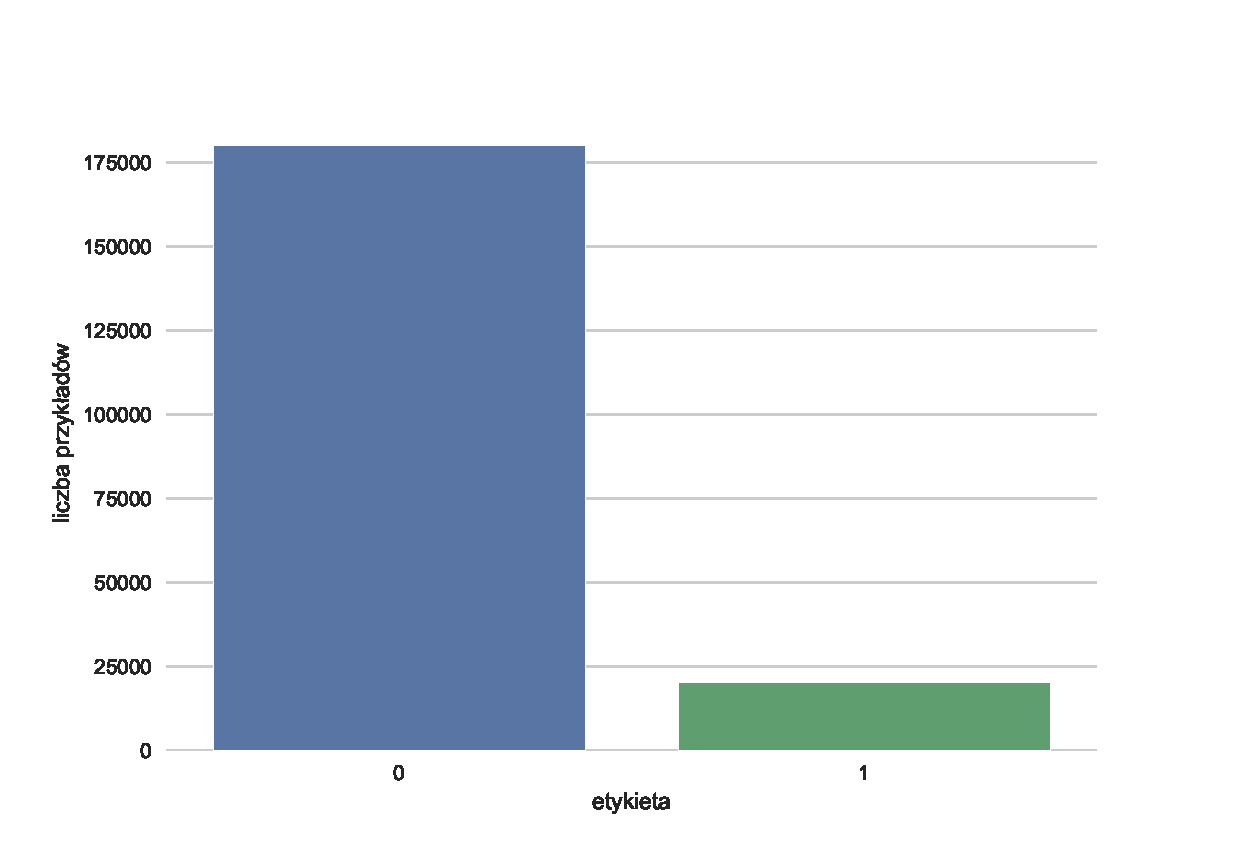
\includegraphics[scale=0.7]{classes.eps}
\caption{Liczba przykładów w każdej z klas}
\label{classescount}
\end{figure}
Jak widać, klasy mocno różnią się licznością, co znacznie podnosi poziom trudności całego zagadnienia.

\subsubsection{EDA (Exploratory Data Analysis)}

Eksploracyjne badanie danych jest podstawowym narzędziem w analizie danych pozwalającym na szczegółowy opis, wizualizację oraz badanie danych bez konieczności zakładania hipotez co do nich. Jest to w głównej mierze metoda oparta o statystykę, a jej wyniki pozwalają na ukierunkowanie kolejnych badań na konkretne cechy posiadanych danych. 
\newline W tablicy \ref{traindescribe} zestawiono dane statystyczne opisujące każdą z cech (kolumny kolejno: nazwa cechy, średnia, odchylenie standardowe, minimum, kwantyl 25\%, mediana, kwantyl 75\%, maksimum) dla zbioru treningowego.

\begin{longtable}{lrrrrrrr}
\toprule
 feature &       mean &        std &      min &        25\% &       50\% &        75\% &      max \\
\midrule
\endhead
\midrule
\multicolumn{8}{r}{{Continued on next page}} \\
\midrule
\caption{Opis cech zbioru treningowego}
\label{traindescribe}
\endfoot

\bottomrule
\endlastfoot
   var\_0 &  10.679914 &   3.040051 &   0.4084 &   8.453850 &  10.52475 &  12.758200 &  20.3150 \\
   var\_1 &  -1.627622 &   4.050044 & -15.0434 &  -4.740025 &  -1.60805 &   1.358625 &  10.3768 \\
   var\_2 &  10.715192 &   2.640894 &   2.1171 &   8.722475 &  10.58000 &  12.516700 &  19.3530 \\
   var\_3 &   6.796529 &   2.043319 &  -0.0402 &   5.254075 &   6.82500 &   8.324100 &  13.1883 \\
   var\_4 &  11.078333 &   1.623150 &   5.0748 &   9.883175 &  11.10825 &  12.261125 &  16.6714 \\
   var\_5 &  -5.065317 &   7.863267 & -32.5626 & -11.200350 &  -4.83315 &   0.924800 &  17.2516 \\
   var\_6 &   5.408949 &   0.866607 &   2.3473 &   4.767700 &   5.38510 &   6.003000 &   8.4477 \\
   var\_7 &  16.545850 &   3.418076 &   5.3497 &  13.943800 &  16.45680 &  19.102900 &  27.6918 \\
   var\_8 &   0.284162 &   3.332634 & -10.5055 &  -2.317800 &   0.39370 &   2.937900 &  10.1513 \\
   var\_9 &   7.567236 &   1.235070 &   3.9705 &   6.618800 &   7.62960 &   8.584425 &  11.1506 \\
  var\_10 &   0.394340 &   5.500793 & -20.7313 &  -3.594950 &   0.48730 &   4.382925 &  18.6702 \\
  var\_11 &  -3.245596 &   5.970253 & -26.0950 &  -7.510600 &  -3.28695 &   0.852825 &  17.1887 \\
  var\_12 &  14.023978 &   0.190059 &  13.4346 &  13.894000 &  14.02550 &  14.164200 &  14.6545 \\
  var\_13 &   8.530232 &   4.639536 &  -6.0111 &   5.072800 &   8.60425 &  12.274775 &  22.3315 \\
  var\_14 &   7.537606 &   2.247908 &   1.0133 &   5.781875 &   7.52030 &   9.270425 &  14.9377 \\
  var\_15 &  14.573126 &   0.411711 &  13.0769 &  14.262800 &  14.57410 &  14.874500 &  15.8633 \\
  var\_16 &   9.333264 &   2.557421 &   0.6351 &   7.452275 &   9.23205 &  11.055900 &  17.9506 \\
  var\_17 &  -5.696731 &   6.712612 & -33.3802 & -10.476225 &  -5.66635 &  -0.810775 &  19.0259 \\
  var\_18 &  15.244013 &   7.851370 & -10.6642 &   9.177950 &  15.19625 &  21.013325 &  41.7480 \\
  var\_19 &  12.438567 &   7.996694 & -12.4025 &   6.276475 &  12.45390 &  18.433300 &  35.1830 \\
  var\_20 &  13.290894 &   5.876254 &  -5.4322 &   8.627800 &  13.19680 &  17.879400 &  31.2859 \\
  var\_21 &  17.257883 &   8.196564 & -10.0890 &  11.551000 &  17.23425 &  23.089050 &  49.0443 \\
  var\_22 &   4.305430 &   2.847958 &  -5.3225 &   2.182400 &   4.27515 &   6.293200 &  14.5945 \\
  var\_23 &   3.019540 &   0.526893 &   1.2098 &   2.634100 &   3.00865 &   3.403800 &   4.8752 \\
  var\_24 &  10.584400 &   3.777245 &  -0.6784 &   7.613000 &  10.38035 &  13.479600 &  25.4460 \\
  var\_25 &  13.667496 &   0.285535 &  12.7200 &  13.456400 &  13.66250 &  13.863700 &  14.6546 \\
  var\_26 &  -4.055133 &   5.922210 & -24.2431 &  -8.321725 &  -4.19690 &  -0.090200 &  15.6751 \\
  var\_27 &  -1.137908 &   1.523714 &  -6.1668 &  -2.307900 &  -1.13210 &   0.015625 &   3.2431 \\
  var\_28 &   5.532980 &   0.783367 &   2.0896 &   4.992100 &   5.53485 &   6.093700 &   8.7874 \\
  var\_29 &   5.053874 &   2.615942 &  -4.7872 &   3.171700 &   4.95020 &   6.798925 &  13.1431 \\
  var\_30 &  -7.687740 &   7.965198 & -34.7984 & -13.766175 &  -7.41175 &  -1.443450 &  15.6515 \\
  var\_31 &  10.393046 &   2.159891 &   2.1406 &   8.870000 &  10.36565 &  11.885000 &  20.1719 \\
  var\_32 &  -0.512886 &   2.587830 &  -8.9861 &  -2.500875 &  -0.49765 &   1.469100 &   6.7871 \\
  var\_33 &  14.774147 &   4.322325 &   1.5085 &  11.456300 &  14.57600 &  18.097125 &  29.5466 \\
  var\_34 &  11.434250 &   0.541614 &   9.8169 &  11.032300 &  11.43520 &  11.844400 &  13.2878 \\
  var\_35 &   3.842499 &   5.179559 & -16.5136 &   0.116975 &   3.91775 &   7.487725 &  21.5289 \\
  var\_36 &   2.187230 &   3.119978 &  -8.0951 &  -0.007125 &   2.19800 &   4.460400 &  14.2456 \\
  var\_37 &   5.868899 &   2.249730 &  -1.1834 &   4.125475 &   5.90065 &   7.542400 &  11.8638 \\
  var\_38 &  10.642131 &   4.278903 &  -6.3371 &   7.591050 &  10.56270 &  13.598925 &  29.8235 \\
  var\_39 &   0.662956 &   4.068845 & -14.5457 &  -2.199500 &   0.67230 &   3.637825 &  15.3223 \\
  var\_40 &  -6.725505 &   8.279259 & -35.2117 & -12.831825 &  -6.61745 &  -0.880875 &  18.1056 \\
  var\_41 &   9.299858 &   5.938088 &  -8.5359 &   4.519575 &   9.16265 &  13.754800 &  26.1658 \\
  var\_42 &  11.222356 &   0.695991 &   8.8590 &  10.713200 &  11.24340 &  11.756900 &  13.4696 \\
  var\_43 &  11.569954 &   0.309599 &  10.6528 &  11.343800 &  11.56500 &  11.804600 &  12.5779 \\
  var\_44 &   8.948289 &   5.903073 &  -9.9396 &   5.313650 &   9.43720 &  13.087300 &  34.1961 \\
  var\_45 & -12.699667 &  21.404912 & -90.2525 & -28.730700 & -12.54720 &   3.150525 &  62.0844 \\
  var\_46 &  11.326488 &   2.860511 &   1.2062 &   9.248750 &  11.31075 &  13.318300 &  21.2939 \\
  var\_47 & -12.471737 &  10.579862 & -47.6862 & -20.654525 & -12.48240 &  -4.244525 &  20.6854 \\
  var\_48 &  14.704713 &  11.384332 & -23.9022 &   6.351975 &  14.55920 &  23.028650 &  54.2738 \\
  var\_49 &  16.682499 &   7.855762 &  -8.0707 &  10.653475 &  16.67240 &  22.549050 &  41.1530 \\
  var\_50 &  12.740986 &   0.691709 &  10.3855 &  12.269000 &  12.74560 &  13.234500 &  15.3172 \\
  var\_51 &  13.428912 &   8.187306 & -15.0462 &   7.267625 &  13.44440 &  19.385650 &  40.6890 \\
  var\_52 &  -2.528816 &   4.985532 & -24.7214 &  -6.065025 &  -2.50245 &   0.944350 &  17.0968 \\
  var\_53 &   6.008569 &   0.764753 &   3.3449 &   5.435600 &   6.02780 &   6.542900 &   8.2315 \\
  var\_54 &   1.137117 &   8.414241 & -26.7786 &  -5.147625 &   1.27405 &   7.401825 &  28.5724 \\
  var\_55 &  12.745852 &   5.690072 &  -3.7826 &   8.163900 &  12.59410 &  17.086625 &  29.0921 \\
  var\_56 &  16.629165 &   3.540174 &   2.7618 &  14.097875 &  16.64815 &  19.289700 &  29.0741 \\
  var\_57 &   6.272014 &   0.795026 &   3.4423 &   5.687500 &   6.26250 &   6.845000 &   9.1609 \\
  var\_58 &   3.177633 &   4.296686 & -12.6009 &   0.183500 &   3.17010 &   6.209700 &  20.4833 \\
  var\_59 &   8.931124 &   0.854798 &   6.1840 &   8.312400 &   8.90100 &   9.566525 &  11.9867 \\
  var\_60 &  12.155618 &   4.222389 &  -2.1006 &   8.912750 &  12.06435 &  15.116500 &  25.1955 \\
  var\_61 & -11.946744 &  11.622948 & -48.8027 & -20.901725 & -11.89200 &  -3.225450 &  27.1029 \\
  var\_62 &   0.874170 &   2.026238 &  -6.3289 &  -0.572400 &   0.79470 &   2.228200 &   7.7536 \\
  var\_63 &   0.661173 &   3.113089 & -10.5544 &  -1.588700 &   0.68170 &   3.020300 &  11.2317 \\
  var\_64 &   6.369157 &   1.485854 &   1.6117 &   5.293500 &   6.37770 &   7.490600 &  11.1537 \\
  var\_65 &   0.982891 &   3.786493 & -14.0888 &  -1.702800 &   1.02135 &   3.739200 &  15.7313 \\
  var\_66 &   5.794039 &   1.121366 &   1.3368 &   4.973800 &   5.78200 &   6.586200 &   9.7132 \\
  var\_67 &  11.943223 &   7.365115 & -19.5443 &   6.753200 &  11.92200 &  17.037650 &  39.3968 \\
  var\_68 &   5.018893 &   0.007186 &   4.9938 &   5.014000 &   5.01910 &   5.024100 &   5.0469 \\
  var\_69 &  -3.331515 &   3.955723 & -16.3094 &  -6.336625 &  -3.32550 &  -0.498875 &   8.5473 \\
  var\_70 &  24.446811 &  11.951742 & -17.0275 &  15.256625 &  24.44500 &  33.633150 &  64.4644 \\
  var\_71 &   0.669756 &   0.266696 &  -0.2240 &   0.472300 &   0.66840 &   0.864400 &   1.5719 \\
  var\_72 &   0.640553 &   3.944703 & -12.3834 &  -2.197100 &   0.64645 &   3.510700 &  14.1500 \\
  var\_73 &  19.610888 &   7.466303 &  -1.6658 &  14.097275 &  19.30975 &  25.207125 &  44.5361 \\
  var\_74 &  19.518846 &  14.112591 & -34.1015 &   9.595975 &  19.53665 &  29.620700 &  70.2720 \\
  var\_75 &  16.853732 &   6.055322 &  -1.2936 &  12.480975 &  16.84420 &  21.432225 &  36.1567 \\
  var\_76 &   6.050871 &   7.938351 & -21.6333 &   0.596300 &   6.29780 &  11.818800 &  34.4352 \\
  var\_77 &  19.066993 &   3.817292 &   7.4257 &  16.014700 &  18.96785 &  22.041100 &  30.9569 \\
  var\_78 &   5.349479 &   1.993792 &  -1.8183 &   3.817275 &   5.44005 &   6.867200 &  11.3507 \\
  var\_79 &  14.402136 &   1.309055 &  10.4454 &  13.375400 &  14.38885 &  15.383100 &  18.2256 \\
  var\_80 &   5.795044 &   7.436737 & -18.0422 &   0.694475 &   6.06175 &  11.449125 &  30.4769 \\
  var\_81 &  14.719024 &   2.299567 &   7.5865 &  13.214775 &  14.84450 &  16.340800 &  23.1324 \\
  var\_82 &  -3.471273 &   8.479255 & -30.0266 & -10.004950 &  -3.28445 &   3.101725 &  21.8934 \\
  var\_83 &   1.025817 &   8.297229 & -24.2201 &  -5.106400 &   1.06970 &   7.449900 &  27.7143 \\
  var\_84 &  -2.590209 &   6.225305 & -24.4398 &  -7.216125 &  -2.51795 &   1.986700 &  17.7424 \\
  var\_85 &  18.362721 &   3.908536 &   7.0230 &  15.338575 &  18.29645 &  21.358850 &  32.9011 \\
  var\_86 &   5.621058 &   7.751142 & -19.2722 &   0.407550 &   6.00670 &  11.158375 &  34.5637 \\
  var\_87 &  11.351483 &   5.661867 &  -8.4816 &   7.247175 &  11.28800 &  15.433225 &  33.3541 \\
  var\_88 &   8.702924 &   2.491460 &   1.3502 &   6.918775 &   8.61620 &  10.567025 &  17.4594 \\
  var\_89 &   3.725208 &   3.560554 &  -9.6014 &   1.140500 &   3.64255 &   6.146200 &  15.4816 \\
  var\_90 & -16.548147 &  13.152810 & -61.7180 & -26.665600 & -16.48260 &  -6.409375 &  27.2713 \\
  var\_91 &   6.987541 &   0.152641 &   6.5218 &   6.869900 &   6.98650 &   7.101400 &   7.4895 \\
  var\_92 &  12.739578 &   4.186252 &  -1.0185 &   9.670300 &  12.67350 &  15.840225 &  26.9976 \\
  var\_93 &  10.556740 &   0.543341 &   8.4916 &  10.195600 &  10.58220 &  10.944900 &  12.5343 \\
  var\_94 &  10.999162 &   2.768099 &   2.8190 &   8.828000 &  10.98385 &  13.089100 &  18.9750 \\
  var\_95 &  -0.084344 &   0.621125 &  -2.4324 &  -0.527400 &  -0.09860 &   0.329100 &   1.8040 \\
  var\_96 &  14.400433 &   8.525400 & -12.1584 &   7.796950 &  14.36990 &  20.819375 &  40.8806 \\
  var\_97 &  18.539645 &  12.642382 & -21.7400 &   8.919525 &  18.50215 &  28.158975 &  58.2879 \\
  var\_98 &   1.752012 &   0.715836 &  -0.6035 &   1.267675 &   1.76830 &   2.260900 &   4.5028 \\
  var\_99 &  -0.746296 &   1.862550 &  -7.2806 &  -2.106200 &  -0.77130 &   0.528500 &   5.0764 \\
 var\_100 &  -6.600518 &   9.181683 & -39.1791 & -13.198700 &  -6.40150 &   0.132100 &  25.1409 \\
 var\_101 &  13.413526 &   4.950537 &   0.0757 &   9.639800 &  13.38085 &  17.250225 &  28.4594 \\
 var\_102 &  22.294908 &   8.628179 &  -7.3829 &  16.047975 &  22.30685 &  28.682225 &  51.3265 \\
 var\_103 &   1.568393 &   0.185020 &   0.9793 &   1.428900 &   1.56600 &   1.705400 &   2.1887 \\
 var\_104 &  11.509834 &   1.970520 &   4.0846 &  10.097900 &  11.49795 &  12.902100 &  19.0206 \\
 var\_105 &   4.244744 &   0.855698 &   0.7153 &   3.639600 &   4.22450 &   4.822200 &   7.1692 \\
 var\_106 &   8.617657 &   1.894899 &   0.9424 &   7.282300 &   8.60515 &   9.928900 &  15.3074 \\
 var\_107 &  17.796266 &   7.604723 &  -5.8980 &  12.168075 &  17.57320 &  23.348600 &  46.3795 \\
 var\_108 &  14.224435 &   0.171091 &  13.7290 &  14.098900 &  14.22660 &  14.361800 &  14.7430 \\
 var\_109 &  18.458001 &   4.355031 &   5.7697 &  15.107175 &  18.28135 &  21.852900 &  32.0591 \\
 var\_110 &   5.513238 &   3.823253 &  -9.2398 &   2.817475 &   5.39430 &   8.104325 &  19.5193 \\
 var\_111 &   6.312603 &   1.082404 &   2.1942 &   5.510100 &   6.34010 &   7.080300 &   9.8002 \\
 var\_112 &   3.317843 &   1.591170 &  -2.0302 &   2.092675 &   3.40840 &   4.577400 &   8.4317 \\
 var\_113 &   8.136542 &   4.459077 &  -5.5139 &   4.803250 &   8.14855 &  11.596200 &  21.5421 \\
 var\_114 &   3.081191 &   0.985396 &  -0.0505 &   2.388775 &   3.08380 &   3.811900 &   6.5850 \\
 var\_115 &   2.213717 &   2.621851 &  -6.8586 &   0.399700 &   2.24985 &   4.121500 &  11.9504 \\
 var\_116 &   2.402570 &   1.650912 &  -3.1630 &   1.171875 &   2.45630 &   3.665100 &   8.1207 \\
 var\_117 &  16.102233 &  13.297662 & -31.8369 &   6.373500 &  15.94485 &  25.780825 &  64.8109 \\
 var\_118 &  -5.305132 &   8.799268 & -37.5277 & -11.587850 &  -5.18950 &   0.971800 &  25.2635 \\
 var\_119 &   3.032849 &   4.182796 &  -9.7742 &  -0.161975 &   3.02395 &   6.098400 &  15.6885 \\
 var\_120 &  24.521078 &  12.121016 & -18.6962 &  15.696275 &  24.35470 &  33.105275 &  74.0321 \\
 var\_121 &  11.310591 &   1.714416 &   6.3052 &   9.996400 &  11.23970 &  12.619425 &  17.3074 \\
 var\_122 &   1.192984 &   5.168479 & -15.1940 &  -2.565200 &   1.20070 &   5.091700 &  18.4714 \\
 var\_123 &   7.076254 &   6.147345 & -12.4059 &   2.817050 &   7.23430 &  11.734750 &  26.8749 \\
 var\_124 &   4.272740 &   2.736821 &  -7.0538 &   2.353600 &   4.30210 &   6.192200 &  14.9915 \\
 var\_125 &  12.489165 &   0.318100 &  11.4861 &  12.245400 &  12.48630 &  12.718100 &  13.6642 \\
 var\_126 &  13.202326 &   0.776056 &  11.2654 &  12.608400 &  13.16680 &  13.811700 &  15.5156 \\
 var\_127 &   0.851507 &   3.137684 &  -8.8769 &  -1.502325 &   0.92500 &   3.293000 &  10.5976 \\
 var\_128 &  -1.127952 &   3.238043 & -11.7559 &  -3.580725 &  -1.10175 &   1.351700 &   9.8096 \\
 var\_129 &  15.460314 &   4.136453 &   2.1863 &  12.514475 &  15.42680 &  18.480400 &  31.2036 \\
 var\_130 &  12.257151 &   0.832199 &   9.5283 &  11.619300 &  12.26465 &  12.876700 &  14.9895 \\
 var\_131 &   0.544674 &   0.456280 &  -0.9548 &   0.207800 &   0.55660 &   0.901000 &   2.1923 \\
 var\_132 &   7.799676 &   1.456486 &   2.8900 &   6.724375 &   7.80910 &   8.911425 &  12.4650 \\
 var\_133 &   6.813270 &   0.375603 &   5.3593 &   6.543500 &   6.80670 &   7.070800 &   8.3091 \\
 var\_134 &  -4.826053 &   6.166126 & -24.2546 &  -9.625700 &  -4.70425 &  -0.178800 &  12.7236 \\
 var\_135 &  -4.259472 &   7.617732 & -31.3808 &  -9.957100 &  -4.11190 &   1.125950 &  21.4128 \\
 var\_136 &  22.968602 &  10.382235 &  -9.9493 &  14.933900 &  22.94830 &  31.042425 &  54.5794 \\
 var\_137 &  17.613651 &   8.890516 &  -9.8510 &  10.656550 &  17.25725 &  24.426025 &  44.4376 \\
 var\_138 &   1.210792 &   4.551750 & -16.4684 &  -2.011825 &   1.21175 &   4.391225 &  18.8187 \\
 var\_139 &   7.760193 &   7.686433 & -21.2743 &   2.387575 &   8.06625 &  13.232525 &  36.0971 \\
 var\_140 &   3.423636 &   4.896325 & -15.4595 &  -0.121700 &   3.56470 &   7.078525 &  21.1219 \\
 var\_141 &   2.897596 &   6.715637 & -16.6937 &  -2.153725 &   2.97550 &   8.192425 &  23.9658 \\
 var\_142 &  11.983489 &   5.691936 &  -7.1080 &   7.900000 &  11.85590 &  16.073925 &  32.8911 \\
 var\_143 &  12.333698 &   2.934706 &   2.8068 &  10.311200 &  12.35635 &  14.461050 &  22.6916 \\
 var\_144 &   8.647632 &   0.922469 &   5.4443 &   7.968075 &   8.65185 &   9.315000 &  11.8101 \\
 var\_145 &   4.841328 &   3.899281 &  -8.2734 &   1.885875 &   4.90470 &   7.676925 &  16.0083 \\
 var\_146 &  10.341178 &   2.518883 &   0.4274 &   8.646900 &  10.39560 &  12.113225 &  20.4373 \\
 var\_147 &  -3.300779 &   7.413301 & -29.9840 &  -8.751450 &  -3.17870 &   2.028275 &  22.1494 \\
 var\_148 &   3.990726 &   0.199192 &   3.3205 &   3.853600 &   3.99600 &   4.131600 &   4.7528 \\
 var\_149 &   5.296237 &  10.385133 & -41.1683 &  -1.903200 &   5.28325 &  12.688225 &  48.4240 \\
 var\_150 &  16.817671 &   2.464157 &   9.2420 &  14.952200 &  16.73695 &  18.682500 &  25.4357 \\
 var\_151 &  10.141542 &   3.962426 &  -2.1915 &   7.064600 &  10.12790 &  13.057600 &  21.1245 \\
 var\_152 &   7.633199 &   3.005373 &  -2.8800 &   5.567900 &   7.67370 &   9.817300 &  18.3846 \\
 var\_153 &  16.727902 &   2.014200 &  11.0308 &  15.233000 &  16.64975 &  18.263900 &  24.0075 \\
 var\_154 &   6.974955 &   4.961678 &  -8.1966 &   3.339900 &   6.99405 &  10.766350 &  23.2428 \\
 var\_155 &  -2.074128 &   5.771261 & -21.8409 &  -6.266025 &  -2.06610 &   1.891750 &  16.8316 \\
 var\_156 &  13.209272 &   0.955140 &   9.9965 &  12.475100 &  13.18430 &  13.929300 &  16.4970 \\
 var\_157 &  -4.813552 &   5.570272 & -22.9904 &  -8.939950 &  -4.86840 &  -0.988575 &  11.9721 \\
 var\_158 &  17.914591 &   7.885579 &  -4.5544 &  12.109200 &  17.63045 &  23.875325 &  44.7795 \\
 var\_159 &  10.223282 &   4.122912 &  -4.6416 &   7.243525 &  10.21755 &  13.094525 &  25.1200 \\
 var\_160 &  24.259300 &  10.880263 &  -7.4522 &  15.696125 &  23.86450 &  32.622850 &  58.3942 \\
 var\_161 &   5.633293 &   0.217938 &   4.8526 &   5.470500 &   5.63350 &   5.792000 &   6.3099 \\
 var\_162 &   5.362896 &   1.419612 &   0.6231 &   4.326100 &   5.35970 &   6.371200 &  10.1344 \\
 var\_163 &  11.002170 &   5.262056 &  -6.5317 &   7.029600 &  10.78870 &  14.623900 &  27.5648 \\
 var\_164 &  -2.871906 &   5.457784 & -19.9977 &  -7.094025 &  -2.63780 &   1.323600 &  12.1193 \\
 var\_165 &  19.315753 &   5.024182 &   3.8167 &  15.744550 &  19.27080 &  23.024025 &  38.3322 \\
 var\_166 &   2.963335 &   0.369684 &   1.8512 &   2.699000 &   2.96020 &   3.241500 &   4.2204 \\
 var\_167 &  -4.151155 &   7.798020 & -35.9695 &  -9.643100 &  -4.01160 &   1.318725 &  21.2766 \\
 var\_168 &   4.937124 &   3.105986 &  -5.2502 &   2.703200 &   4.76160 &   7.020025 &  14.8861 \\
 var\_169 &   5.636008 &   0.369437 &   4.2588 &   5.374600 &   5.63430 &   5.905400 &   7.0890 \\
 var\_170 &  -0.004962 &   4.424621 & -14.5060 &  -3.258500 &   0.00280 &   3.096400 &  16.7319 \\
 var\_171 &  -0.831777 &   5.378008 & -22.4793 &  -4.720350 &  -0.80735 &   2.956800 &  17.9173 \\
 var\_172 &  19.817094 &   8.674171 & -11.4533 &  13.731775 &  19.74800 &  25.907725 &  53.5919 \\
 var\_173 &  -0.677967 &   5.966674 & -22.7487 &  -5.009525 &  -0.56975 &   3.619900 &  18.8554 \\
 var\_174 &  20.210677 &   7.136427 &  -2.9953 &  15.064600 &  20.20610 &  25.641225 &  43.5468 \\
 var\_175 &  11.640613 &   2.892167 &   3.2415 &   9.371600 &  11.67980 &  13.745500 &  20.8548 \\
 var\_176 &  -2.799585 &   7.513939 & -29.1165 &  -8.386500 &  -2.53845 &   2.704400 &  20.2452 \\
 var\_177 &  11.882933 &   2.628895 &   4.9521 &   9.808675 &  11.73725 &  13.931300 &  20.5965 \\
 var\_178 &  -1.014064 &   8.579810 & -29.2734 &  -7.395700 &  -0.94205 &   5.338750 &  29.8413 \\
 var\_179 &   2.591444 &   2.798956 &  -7.8561 &   0.625575 &   2.51230 &   4.391125 &  13.4487 \\
 var\_180 &  -2.741666 &   5.261243 & -22.0374 &  -6.673900 &  -2.68880 &   0.996200 &  12.7505 \\
 var\_181 &  10.085518 &   1.371862 &   5.4165 &   9.084700 &  10.03605 &  11.011300 &  14.3939 \\
 var\_182 &   0.719109 &   8.963434 & -26.0011 &  -6.064425 &   0.72020 &   7.499175 &  29.2487 \\
 var\_183 &   8.769088 &   4.474924 &  -4.8082 &   5.423100 &   8.60000 &  12.127425 &  23.7049 \\
 var\_184 &  12.756676 &   9.318280 & -18.4897 &   5.663300 &  12.52100 &  19.456150 &  44.3634 \\
 var\_185 &  -3.983261 &   4.725167 & -22.5833 &  -7.360000 &  -3.94695 &  -0.590650 &  12.9975 \\
 var\_186 &   8.970274 &   3.189759 &  -3.0223 &   6.715200 &   8.90215 &  11.193800 &  21.7392 \\
 var\_187 & -10.335043 &  11.574708 & -47.7536 & -19.205125 & -10.20975 &  -1.466000 &  22.7861 \\
 var\_188 &  15.377174 &   3.944604 &   4.4123 &  12.501550 &  15.23945 &  18.345225 &  29.3303 \\
 var\_189 &   0.746072 &   0.976348 &  -2.5543 &   0.014900 &   0.74260 &   1.482900 &   4.0341 \\
 var\_190 &   3.234440 &   4.559922 & -14.0933 &  -0.058825 &   3.20360 &   6.406200 &  18.4409 \\
 var\_191 &   7.438408 &   3.023272 &  -2.6917 &   5.157400 &   7.34775 &   9.512525 &  16.7165 \\
 var\_192 &   1.927839 &   1.478423 &  -3.8145 &   0.889775 &   1.90130 &   2.949500 &   8.4024 \\
 var\_193 &   3.331774 &   3.992030 & -11.7834 &   0.584600 &   3.39635 &   6.205800 &  18.2818 \\
 var\_194 &  17.993784 &   3.135162 &   8.6944 &  15.629800 &  17.95795 &  20.396525 &  27.9288 \\
 var\_195 &  -0.142088 &   1.429372 &  -5.2610 &  -1.170700 &  -0.17270 &   0.829600 &   4.2729 \\
 var\_196 &   2.303335 &   5.454369 & -14.2096 &  -1.946925 &   2.40890 &   6.556725 &  18.3215 \\
 var\_197 &   8.908158 &   0.921625 &   5.9606 &   8.252800 &   8.88820 &   9.593300 &  12.0004 \\
 var\_198 &  15.870720 &   3.010945 &   6.2993 &  13.829700 &  15.93405 &  18.064725 &  26.0791 \\
 var\_199 &  -3.326537 &  10.438015 & -38.8528 & -11.208475 &  -2.81955 &   4.836800 &  28.5007 \\
\end{longtable}

Z tabeli \ref{traindescribe} wynika, że odchylenie standardowe dużej liczby cech jest znaczne. Kolejną obserwacją jest podobny zakres wartości danych każdej cechy. Wszystkie wartości ze zbioru treningowego mieszczą się w zakresie $[-91, 75]$, co jest zaskakująco małym przedziałem dla tak dużej liczby cech. Za to średnie wartości poszczególnych atrybutów są bardzo zróżnicowane i wynoszą od $-16.5$ do $24.5$. Warto zwrócić uwagę na zmienną o numerze $68$, dla której minimum wynosi 5.018893, a maksimum 5.0469 (odchylenie standardowe: 0.007186). Jest to cecha o najmniejszym rozstrzale wartości.
\newline 

Istotny może być również rozkład wartości poszczególnych cech w zależności od klasy.
Rysunek \ref{featuresDistribution25} przedstawia wizualizację tychże rozkładów dla pierwszych 25 cech (w zbiorze treningowym). Wykresy dla wszystkich 200 kolumn znajdują się w załączonym pliku \textit{AllFeaturesDistribution.png}.

\begin{figure}[H]
\centering 
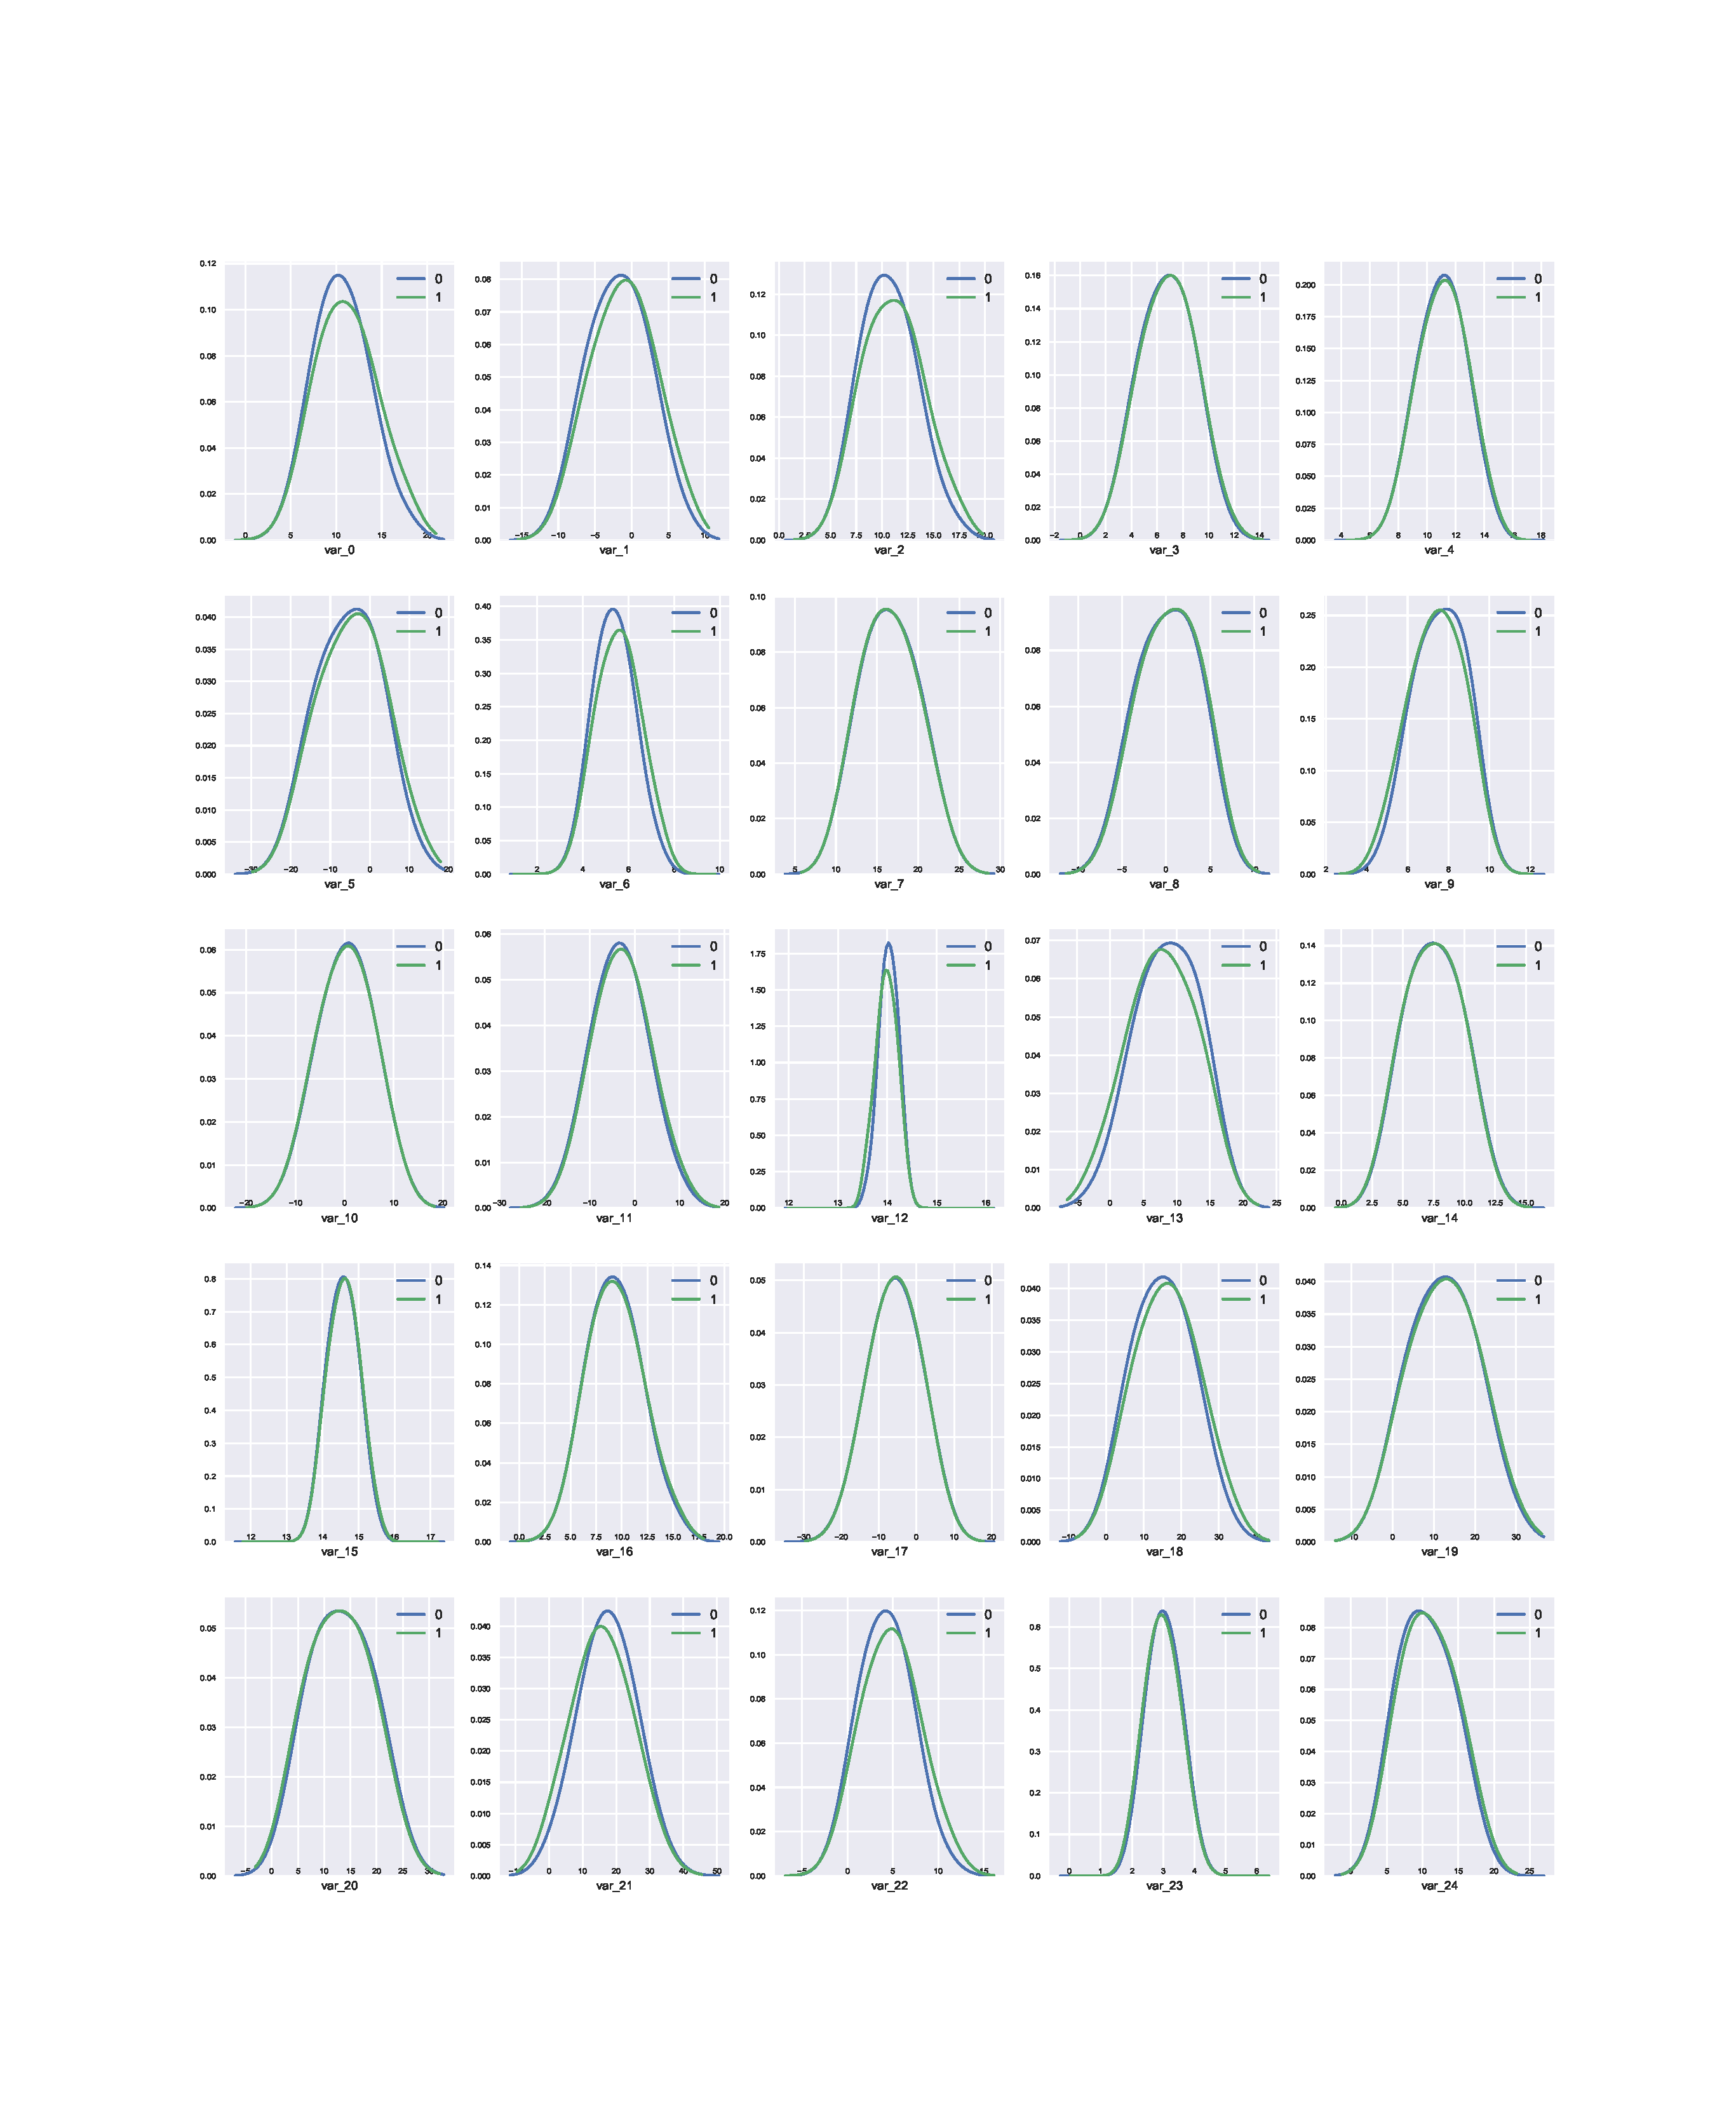
\includegraphics[width = 472pt]{feature_distribution.eps}
\caption{Rozkład wartości pierwszych 25 cech w podziale na klasy (dotyczy zbioru treningowego)}
\label{featuresDistribution25}
\end{figure}

Wnioskując z omawianych wizualizacji, rozkład wartości jest zbliżony w obu klasach dla wszystkich rozważanych kolumn i ma charakter rozkładu Gaussa. Wykresy odpowiadające obu klasom niemalże pokrywają się. Jednak część cech (np. dla var0, var2, var6 itd.) charakteryzuje się delikatnymi rozbieżnościami. Można wnioskować, że będą one szczególnie istotne w procesie klasyfikacji.

Aby porównać istotność cech pod omawianym względem i uszeregować je od najistotniejszej (dla klasyfikatora) do wnoszącej najmniej informacji, potrzebujemy pewnej metryki opisującej różnicę w rozkładzie wartości danej cechy w zależności od klasy.   
\newline Oznaczmy jako $Z_0$ figurę składającą się ze wszystkich punktów pod wykresem rozkładu wartości dla klasy 0. Analogicznie, jako $Z_1$ oznaczmy figurę składającą się ze wszystkich punktów pod wykresem rozkładu wartości dla klasy 1.
\newline Jako wartość metryki opisującej różnicę rozkładów przyjmujemy pole powierzchni figury będącej wynikiem różnicy symetrycznej figur $Z_0$ i $Z_1$. Czym większe pole, tym bardziej rozbieżne są rozkłady wartości poszczególnych klas. A czym bardziej rozbieżne rozkłady, tym (potencjalnie) wartościowsza jest dana kolumna.
\newline Tabela \ref{tab:my_label} zawiera zestawienie 20 kolumn potencjalnie najbardziej przydatnych w procesie klasyfikacji pod omawianym względem. Różnice zostały zaokrąglone do części dziesięciotysięcznych. Pełne zestawienie cech znajduje się w pliku \textit{feature\_distribution\_differences.csv}.

\begin{table}[H]
    \centering
    \begin{tabular}{|c|c|}
    \hline
    feature & difference \\
    \hline
    \hline
    var\_68 &	6.0303 \\
    \hline
    var\_12 &	5.7848 \\
    \hline
    var\_166 &	4.7379 \\
    \hline
    var\_23	& 4.4199 \\
    \hline
    var\_148	& 4.1119 \\
    \hline
    var\_108	& 3.7552 \\
    \hline
    var\_169	& 3.3483 \\
    \hline
    var\_28	& 2.8039 \\
    \hline
    var\_57	& 2.7702 \\
    \hline
    var\_43	& 2.6340 \\
    \hline
    var\_133	& 2.5368 \\
    \hline
    var\_91	& 2.2162 \\
    \hline
    var\_53	& 2.2148 \\
    \hline
    var\_6	& 1.9670 \\
    \hline
    var\_95	& 1.9046 \\
    \hline
    var\_111	& 1.8731 \\
    \hline
    var\_125	& 1.8327 \\
    \hline
    var\_156	& 1.7606 \\
    \hline
    var\_105	& 1.7261 \\
    \hline
    var\_93	& 1.6879 \\
    \hline
    \end{tabular}
    \caption{20 cech zbioru treningowego charakteryzujących się największą rozbieżnością pod względem rozkładu klas}
    \label{tab:my_label}
\end{table}

Warto też porównać rozkład cech zbioru treningowego i testowego. Wizualizacja dla pierwszych 25 cech została przedstawiona na rysunku \ref{features_distribution_train_vs_test}.

\begin{figure}[H]
\centering 
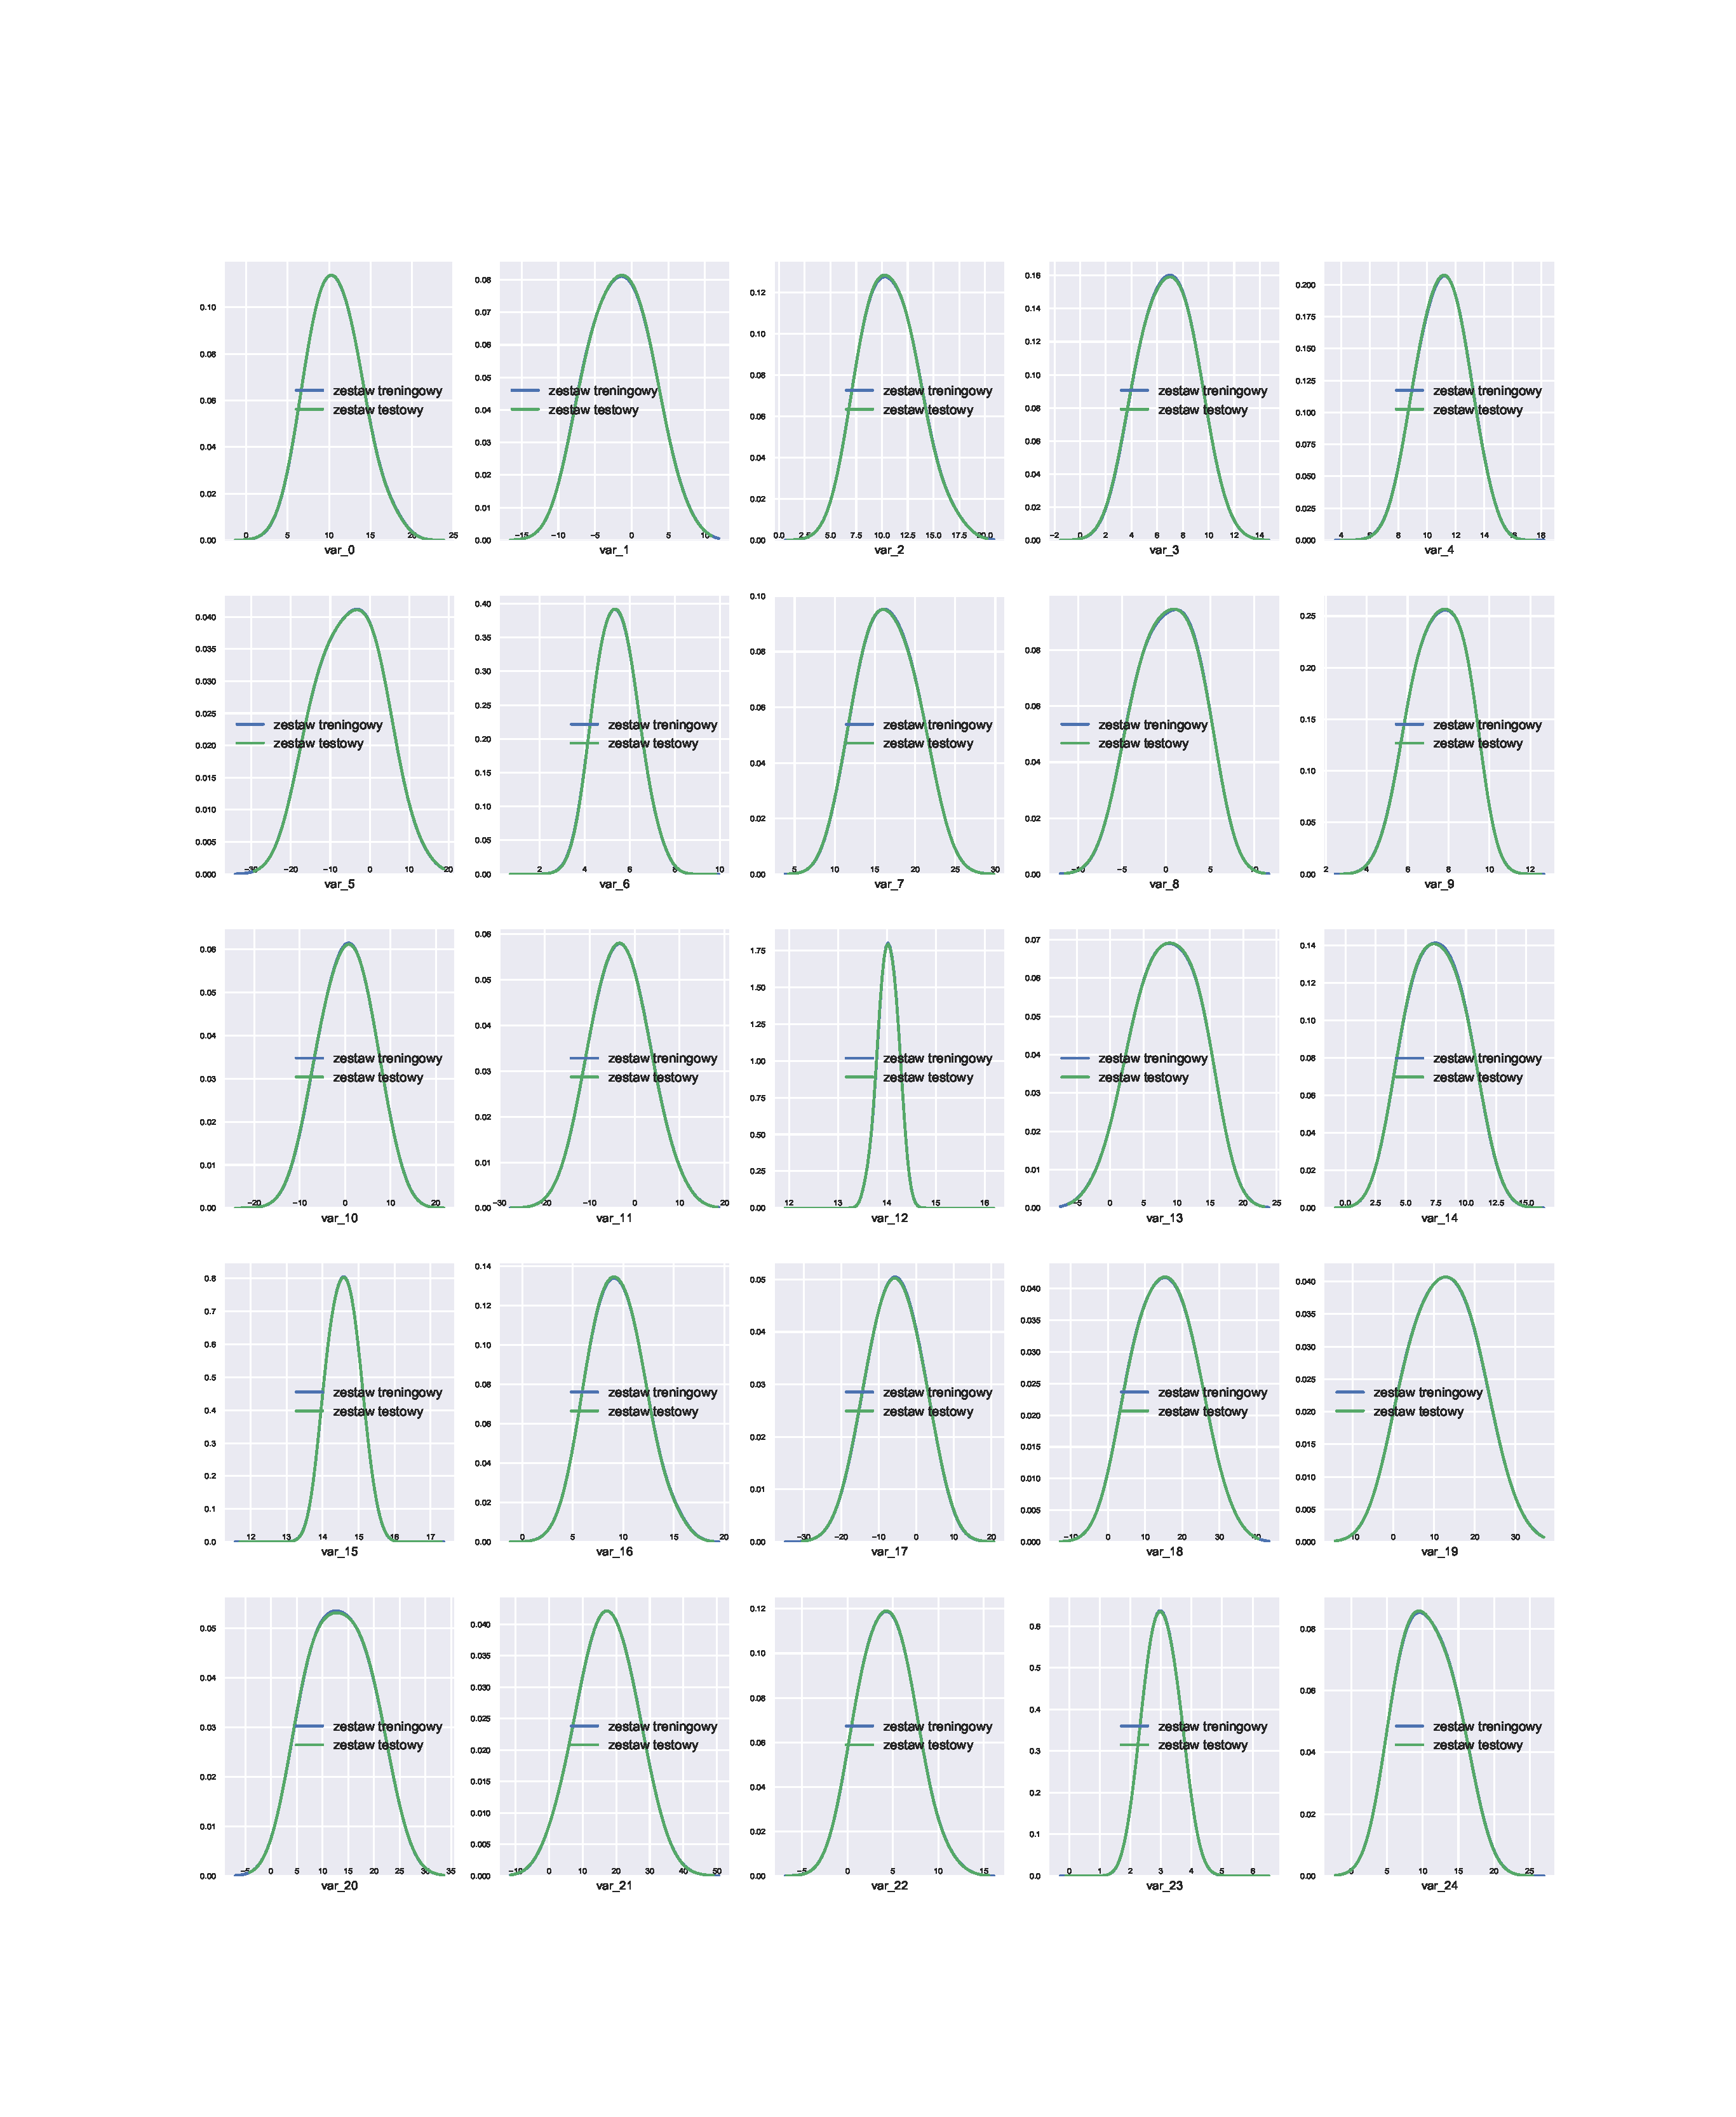
\includegraphics[width = 472pt]{feature_distribution_train_vs_test.eps}
\caption{Rozkład wartości pierwszych 25 cech w zbiorze treningowym i testowym}
\label{features_distribution_train_vs_test}
\end{figure}

Jak można zauważyć, zbiory testowy i treningowy są łudząco podobne pod względem dystrybucji wartości poszczególnych zmiennych. Stanowi to dużą zaletę. Prawdopodobnie wykorzystanie informacji z kolumn o największych rozbieżnościach przy podziale na klasy (w zbiorze treningowym) przyniesie sukces również w przypadku zbioru testowego.

\subsubsection{PCA (Principal Component Analysis)}
PCA sciśle wiąże się z metodami wyboru cech i algorytmami, które ten wybór realizują.
Dane składają się z 200 cech liczbowych, dlatego warto sprawdzić, czy wszystkie wprowadzają nową informację. Może się tak zdarzyć, że niektóre z tych cech są ze sobą skorelowane na tyle, że można niektóre z nich pominąć w modelu, nie tracąc na jego jakości. Co więcej, użycie wszystkich dostępnych cech może dać w rezultacie gorsze wyniki niż użycie podzbioru zbioru cech. W celu zbadania, które z dostępnych cech mają istotny wpływ na dany problem przeprowadza się analizę PCA. Celem takiej analizy jest znalezienie zbioru cech, których użycie zmaksymalizuje jakość modelu przy jednoczesnym zminimalizowaniu zbioru cech użytych w danym problemie.
\newline
Na poniżej została zaprezentowana macierz korelacji cech zbioru testowego.
\begin{figure}[H]
\centering 
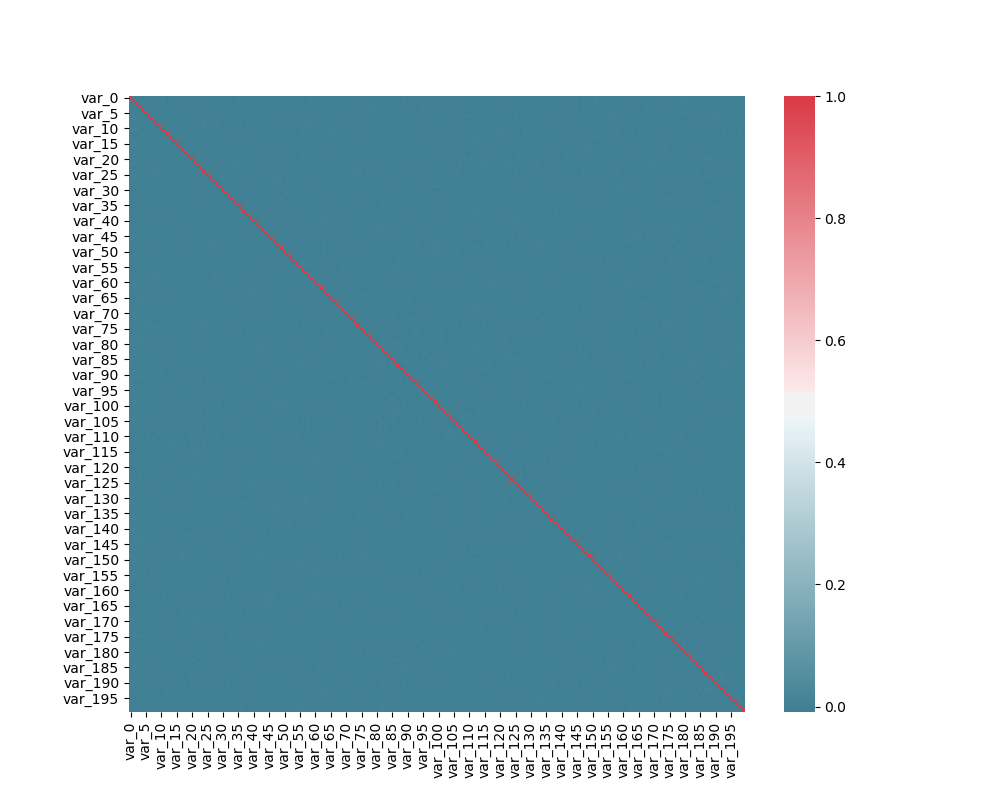
\includegraphics[width = 472pt]{feature_correlation_matrix}
\caption{Macierz korelacji cech w zbiorze testowym}
\label{feature_correlation_matrix}
\end{figure}

Z powyższego wykresu możemy odczytać, że cechy nie są ze sobą skorelowane lub są w bardzo małym stopniu. \\
\\
\begin{table}[H]
\centering
\begin{tabular}{|c|c|c|}
 \hline
 Cecha 1  & Cecha 2  &        Wartość korelacji \\
    \hline
     \hline
var\_75 & var\_139 &  0.009868 \\
 \hline
var\_96 & var\_143 &  0.008829 \\
 \hline
var\_31 & var\_132 &  0.008714 \\
 \hline
var\_2 & var\_164 &  0.008614 \\
 \hline
var\_122 & var\_164 &  0.008513 \\
 \hline
var\_36 & var\_175 &  0.008424 \\
 \hline
var\_103 & var\_110 &  0.008405 \\
 \hline
var\_40 & var\_163 &  0.008335 \\
 \hline
var\_19 & var\_187 &  0.008201 \\
 \hline
var\_92 & var\_164 &  0.008058 \\
 \hline
\end{tabular}
\caption{10 najbardziej skorelowanych cech.}
\end{table}
Powyższa tabela przedstawiająca 10 najbardziej skorelowanych cech w zbiorze testowym upewnia nas, że wygląd macierzy korelacji przedstawionej na rysunku \ref{feature_correlation_matrix} to nie błąd, a jedynie fakt, że cechy są od siebie niezależne.
Taka informacja nie pozwala nam na odrzucenie niektórych kolumn, ponieważ na wykresie widzimy, że potencjalnie każda cecha wnosi coś nowego i może mieć istotny wpływ na jakość przyszłego modelu.
\newline
Przy użyciu dostępnych bibliotek takich jak \textit{sklearn} w języku Python, można wykonać redukcję wymiarowości problemu przy pomocy dedytkowanej do tego klasy \textit{PCA}. Dzięki niej jesteśmy w stanie zredukować praktycznie dowolnie wymiar zadania, większym lub mniejszym kosztem.
Na przykład przy zachowaniu 95\% wariancji dostępny w bibliotece algorytm redukuje wymiar do 190 cech, co jeszcze bardziej pokazuje, że każda cecha może mieć istotny wpływ na wynik (liniowa zależność zachowania wariancji do ilości cech). Jednak aby się o tym przekonać w 100-u procentach niezbędne będą testy na konkretnych modelach i algorytmach wybranych do rozwiązania tego problemu.


\subsubsection{Outliers}
Dane ze zbioru testowego zostały sprawdzone pod kątem wystąpienia w nich tak zwanych \textit{outliers} (elementy zbioru znacznie odbiegające od pozostałych). Wynik tego sprawdzenia prezentuje poniższy wykres.
\begin{figure}[H]
\centering 
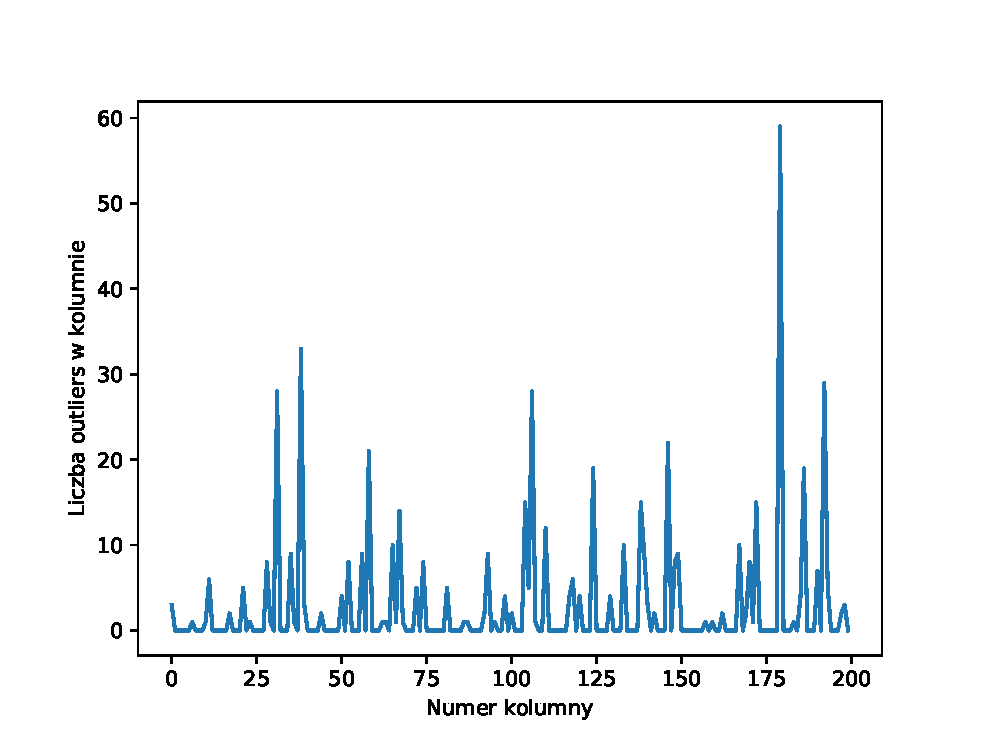
\includegraphics[width = 472pt]{outliers.eps}
\caption{Liczba outliers dla poszczególnych cech zbioru testowego}
\label{outliers}
\end{figure}

Powyższy wykres przedstawia liczbę outliers biorąc pod uwagę wartości z poszczególnych cech(kolumn).
Do przygotowania powyższego wykresu zostało przyjęte założenie, że za outlier-a uznajemy element, którego wartość $x$ danej cechy nie znajduje się w zbiorze $X$.
\begin{center}
Q1, Q3 - odpowiednio pierwszy i trzeci kwartyl rozkładu danej cechy.\\
IQR = Q3-Q1\\
    $X=\{x\in R : x \in \left[Q1-2*IQR, Q3+2*IQR\right]\}$
\end{center}
Z wykresu można odczytać, że dla większości cech outliers nie występują lub ich liczba jest poniżej 10. Tylko w kilku przypadkach liczba outliers przekracza 20 i nie jest wykluczone, że outliers różnych cech pojawiają się dla tego samego elementu zbioru. W odniesieniu do liczności całego zbioru liczba ta jest mała i nie przekracza 1\%. 
\section{Ocena modeli}

Sposób oceny modeli został narzucony przez organizatorów konkursu. Ze względu na nierównomierny podział klas, do oceny modeli wykorzystana jest miara AUC, którą można uzyskać poprzez policzenie pola pod krzywą ROC.


\section{Modele klasyczne}

\section{Modele klasyczne}

\subsection{Regresja SVM}
\subsubsection{Opis metody}
Jednym z modeli dla których podjęto próbę rozwiązania problemu są wektory SVM. Niestety dla danych treningowych, których jest około $200$ tys. przeprowadzenie obliczeń jest praktycznie niemożliwe. Dane zostały zredukowane wykorzystując metodę \textit{undersampling} dzięki której uzyskano koło $40$ tys danych i dodatkowo zachowano balans pomiędzy danymi z odpowiedziami 0 i 1. Dodatkowo dane treningowe i testowe są przeskalowane do przedziału $[0, 1]$, aby przyspieszyć uczenie.

\subsubsection{Testy}
Na samym początku wykonano testy dla różnych kerneli. Wyniki tych testów zostały przedstawione w tabeli nr \ref{tab:svm_kernels}. Dla funkcji jądrowej \textit{rbf} metoda zwróciła najlepszy wynik.
\begin{table}[H]
    \centering
    \begin{tabular}{|c|c|}
    \hline
    Kernel & Wyniki \\
    \hline
    \hline
    \textit{sigmoid} &	0.8524 \\
    \hline
    \textit{linear} &	0.8620 \\
    \hline
    \textit{poly} &	0.8524 \\
    \hline
    \textbf{\textit{rbf}} &	\textbf{0.8629} \\
    \hline
    \end{tabular}
    \caption{Wyniki modelów SCV dla różnych kerneli i domyślnych parametrów (C=1.0, epsilon=0.1, gamma=0.005, degree=3)}
    \label{tab:svm_kernels}
\end{table}

W kolejnych testach sprawdzano działanie modelu zmieniając parametry: eps, C i gamma. Wyniki zostały przedstawione w tabeli nr \ref{tab:rgf_test} Najlepszy wynik jaki udało się uzyskać to 0.8841. Końcowy wynik dla tego modelu jaki uzyskano na koniec konkursu to 0.88079.

\begin{table}[H]
    \centering
    \begin{tabular}{|c|c|c|c|}
    \hline
    Eps & C & Gamma & Wynik \\
    \hline
    \hline
    0.2 & - & - & 0.8628 \\
    \hline
    0.1 & - & - & 0.8629 \\
    \hline
    0.05 & - & - & 0.8618 \\
    \hline
    0.01 & - & - & 0.8603 \\
    \hline
    0.3 & - & - & 0.8590 \\
    \hline
    \textbf{0.15} & - & - & 0.8633 \\
    \hline
    \textbf{0.15} & 2 & - & 0.8564 \\
    \hline
    \textbf{0.15} & 10 & - & 0.8561 \\
    \hline
    \textbf{0.15} & 0.5 & - & 0.8753 \\
    \hline
    \textbf{0.15} & 0.1 & - & 0.8840 \\
    \hline
    \textbf{0.15} & 0.01 & - & 0.8828 \\
    \hline
    \textbf{0.15} & 0.3 & - & 0.8804 \\
    \hline
    \textbf{0.15} & \textbf{0.005} & - & 0.8841 \\
    \hline
    \textbf{0.15} & \textbf{0.005} & 1 & 0.5 \\
    \hline
    \textbf{0.15} & \textbf{0.005} & 10 & 0.5 \\
    \hline
    \textbf{0.15} & \textbf{0.005} & 0.1 & 0.79 \\
    \hline
    \textbf{0.15} & \textbf{0.005} & 0.01 & 0.8838 \\
    \hline
    \textbf{0.15} & \textbf{0.005} & 0.001 & 0.8779 \\
    \hline
    \textbf{0.15} & \textbf{0.005} & \textbf{0.005} & 0.8841 \\
    \hline
    \end{tabular}
    \caption{Wyniki modelów SCV dla kernela \textit{rbf} i różnych parametrów}
    \label{tab:rgf_test}
\end{table}

\subsubsection{Instrukcja uruchomienia SVM}

SVM został zaimplementowany w Pythonie i można go uruchomić jako aplikację konsolową:

\begin{lstlisting}
svr.py [-h] [--kernel KERNEL] [--eps EPS] [--gamma GAMMA] 
		[--c C] [--wsp WSP]
\end{lstlisting}

Znaczenie parametrów:

\begin{itemize}
    \item -h: wyświetlenie pomocy
    \item --kernel: typ kernela wykorzystywanego w algorytmie np.: 'rbf', 'poly', 'linear', 'sigmoid',
    \item --eps: epsilon wykorzystywany w algorytmie SVM,
    \item --gamma: gamma wykorzystywana w algorytmie SVM,
    \item --c: parametr C wykorzystywany w algorytmie SVM,
    \item --wsp: ilość danych użytych do testów wsp $\in [0,1]$.
\end{itemize}
\newpage
Przykład wywołania:
\begin{lstlisting}
python svr.py --wsp=0.1
Namespace(c=1, eps=0.1, gamma='auto', kernel='rbf', wsp=0.1)
Wczytywanie danych
Przeprowadzenie preprocessingu danych trenigowych
Liczba danych:  18000  w tym: [(0, 16242), (1, 1758)]
Liczba danych po zastosowaniu Undersampled: 3516  w tym: [(0, 1758), (1, 1758)]
Rozpoczecie procesu nauki
Przeprowadzenie preprocessingu danych testowych
Rozpoczecie procesu testowania
Przeprowadzenie postprocessingu danych testowych
Otrzymany rezultat: 0.8546027178022656
\end{lstlisting}


\subsection{Sieć neuronowa}

\subsubsection{Opis metody}
Użycie standardowego modelu wielowarstwowej sieci perceptronowej nie przyniosło zadowalających rezultatów. Uzyskany został wynik około 0.85. Okazało się, że użycie konwolucyjnej sieci neuronowej znacznie poprawiło wynik. Sama zmiana modelu sieci pozwoliła na osiągnięcie rezultatu 0.892. Spróbujmy wyjaśnić skąd ta różnica. Poniżej zamieszczony został dokładny model sieci.

\begin{lstlisting}[caption={Model sieci CNN}, captionpos=b]
Layer (type)                 Output Shape              Param #   
=================================================================
conv1d_2 (Conv1D)            (None, 200, 32)           64        
_________________________________________________________________
batch_normalization_2 (Batch (None, 200, 32)           128       
_________________________________________________________________
flatten_2 (Flatten)          (None, 6400)              0         
_________________________________________________________________
dense_2 (Dense)              (None, 1)                 6401      
=================================================================
Total params: 6,593
\end{lstlisting} 

Wejście sieci jest przerabiane na 2 wymiary, tj. ma rozmiar 200x1. 
Zobaczmy, że pierwsza warstwa ma zaledwie 64 parametry (32 filtry rozmiaru 1x1 oraz 32 biasy). Jako funkcja aktywacji została użyta funkcja ReLU. Znaczna część cech po przejściu przez filtr zostanie wyzerowana. Stąd też macierz wynikowa 200x32 jest macierzą rzadką. Warstwa ta pozwala na automatyczne wyodrębnianie ważności cech jednych nad drugimi. Można zauważyć analogię do działanie płytkich modeli boostingu, które są skuteczne dla tego konkursu. Dalej, warstwa normalizująca pozwala na przyspieszenie treningu, nie ma wpływu na poprawę jakości wyniku. Następnie wypłaszczamy macierz do jednego wymiaru uzyskując wektor długości 6400 (zamiast 200 w klasycznym MLP) dla warstwy fully-connected. Dopiero w ostatniej warstwie następuje mieszanie pomiędzy cechami. Zastosowanie funkcji aktywacji sigmoid pozwala na uzyskanie wyniku w przedziale [0,1].

Konwolucja pozwoliła na działanie na każdej z cech niezależnie (przed zastosowaniem warstwy Flatten). Jest to skuteczne, ponieważ de facto nastąpiła próba odzyskania danych oryginalnych przed wstępnym przetworzeniem przez Santander i możliwość podziałania na danych bardziej skorelowanych. 

Ze względu na niezrównoważenie klas do modelu wprowadzono oversampling. Polegało to na nadaniu wag klasom. Taką obsługę oversamplingu dostarcza \textit{keras}, co ostatecznie okazało się delikatnie skuteczniejsze niż samemu generowanie nowych danych. Ponadto zastosowano komitet 30 sieci. Jako rezultat końcowy były brane średnie arytmetyczne z uzyskanych rezultatów sieci. Ostateczny wynik w prywatnym rankingu zawodów wyniósł \textbf{0.89823}, co pozwoliło na zajęcie miejsca w top 49\% najlepszych wyników. Z samego modelu sieci już niewiele dałoby się poprawić. Na uzyskanie lepszego wyniku (powyżej 0.9) potrzebna byłaby dogłębna analiza danych i sensowna rozbudowa wektora cech (feature engineering) z 200 nawet i do 1000. Zajęcie czołowego miejsca w konkursie zależało głównie od jakości EDA.

\subsubsection{Instrukcja uruchomienia}
Sieć neuronowa została zaimplementowana w Pythonie i można ją uruchomić jako aplikację konsolową:
\begin{lstlisting}
cnn.py [-h] [--train_data=PATH] [--data=PATH] [--output=PATH]
\end{lstlisting}
Znaczenie parametrów:

\begin{itemize}
    \item -h: wyświetlenie pomocy
    \item train{\_}data: ścieżka do pliku csv w którym znajdują się dane treningowe. Domyślnie: ../data/train.csv
    \item data: ścieżka do pliku csv w którym znajdują się dane. Domyślnie: ../data/test.csv
    \item output: ścieżka do pliku wyjściowego. Domyślnie: cnnx{\_}submission.csv
\end{itemize}

\section{Modele niekonwencjonalne}

\subsection{Boosting drzew decyzyjnych}

\subsubsection{Opis metody}

Pierwszym niekonwencjonalnym algorytmem użytym jest gradient boosting drzew decyzyjnych. Implementacja metody pochodzi z biblioteki xgboost \cite{xgboost}. Ogólnie metody boostingu polegają na tworzenu komitetu składającego się z wielu słabych klasyfikatorów. Ważne jest tutaj to, że w przypadku boostingu kolejne modele są tworzone sekwencyjnie, późniejsze zależą zatem od poprzednich. To jest główną różnicą do baggingu (czyli np. metoda Random Forest), gdzie modele w komitecie są niezależne od siebie. Tworzenie kolejnych klasyfikatorów, uczonych na błędach poprzednich, może prowadzić do overfittingu, co będzie widoczne przy wynikach.

Jak było wcześniej wspomniane, korzystamy z gradient boostingu, co oznacza, że w procesie uczenia jest minimalizowana pewna funkcja straty za pomocą gradientowych metod optymalizacji. W naszym przypadku tą funkcją optymalizowaną jest entropia binarna:

\begin{equation}
    l(y, p) = -\frac{1}{N} \sum_{i = 1}^{N} \left[ y_i log p_i + (1 - y_i) log (1 - p_i) \right]
\end{equation},
gdzie $y$ jest wektorem prawdziwych wartości do przewidzenia ze zbioru treningowego, $p$ jest wektorem prawdopodobieństw wyznaczonych przez metodę dla danych treningowych, a $N$ jest licznością zbioru treningowego. Funkcja straty ma również drugi składnik, tak zwany składnik regularyzacji, który ma karać złożone modele i tym samym pomóc uniknąć przetrenowania.

W konkursie celem było uzyskanie jak największej miary AUC (powierzchnia pod krzywą ROC). Jednak tak miara nie jest różniczkowalna, dlatego została zastosowana funkcja straty wyżej wymieniona. 

Drzewa używane w tym modelu to są tak zwane drzewa CART (classification and regression trees). Różnią się od zwykłych drzew decyzyjnych tym, że w liściach nie znajduje się klasa, do której należy dany obiekt, lecz pewna wartość (waga), z której można otrzymać prawdopodobieństwo przynależności do jednej z klas.

Metoda posiada wiele hiperparametrów, niemożliwe byłoby znalezienie najlepszej kombinacji, dlatego też hiperparametry były optymalizowane sekwencyjnie. Następujące parametry zostały wzięte pod uwagę:

\begin{enumerate}
    \item scale\_pos\_weight - przez tą wartość są skalowane wartości funkcji straty dla przypadków pozytywnych (czyli tych, których etykietą jest jednyka). Można tego parametru użyć, aby poradzić sobie z niezbalansowanym zbiorem danych, jak w naszym przypadku. Przypadków pozytywnych jest w zbiorze danych około dziewięć razy mniej niż negatywnych, więc otrzymują one wagę dziewięć. Alternatywnym rozwiązaniem do tego, jest użycie oversamplingu do zrównoważenia zbiorów, a następnie trenowanie z scale\_pos\_weight równym jeden. Oba podejścia zostały przetestowane.
    
    \item liczba kolumn użytych do przewidywania - co prawda analiza danych wykazała, ze kolumny są nieskorelowane ze sobą, jednak warto to również sprawdzić w praktyce. Do wybierania najbardziej odpowiednich cech, została użyta metoda ANOVA.
    
    \item maksymalna wysokość drzew decyzyjnych - głębsze drzewa lepiej potrafią oddać strukturę danych treningowych, ale tym samym mogą prowadzić do przetrenowania.
    
    \item min\_child\_weight - parametr sterujący kiedy algorytm przestaje dodawać kolejne liście. Większe wartości powinny powodować, że algorytm będzie bardziej ogólny, nie będzie się uczył dokładnych szczegółów, przez co być może uda się uniknąć przetrenowanie. Za duże wartości z drugiej strony mogą powodować, że model nie będzie w stanie się nauczyć zależności. Ten parametr jest ściśle związany z wysokością drzewa, tak więc oba parametry były optymalizowane jednocześnie. 
    
    \item subsample - frakcja obserwacji wylosowana do tworzenia kolejnego drzewa. Jeżeli wartość tego parametru jest mniejsza niż jeden, to przy tworzeniu drzewa jest losowany tylko pewien procent obserwacji. Mniejsze wartości zatem przeciwdziałają przetrenowaniu, algorytm nie może nauczyć się "na pamięć" całego zbioru treningowego, jak zawsze tylko część widzi.
    
    \item colsample\_by\_tree - parametr bardzo podobny do subsample, tylko że tym razem do tworzenia drzewa jest wybierany tylko pewien podzbiór cech (kolumn). Oba parametry osiągają podobny cel, były zatem równocześnie optymalizowane.
    
    \item eta - współczynnik uczenia dla metody gradientowej. Małe wartości wydłużają proces uczenia, algporytm musi wykonać więcej kroków, jednak za duże wartości mogą spowodować, że poszukiwane optimum lokalne zostanie przeskoczone.
    
    % \item alfa - współczynnik regularyzacji L1, lambda - współczynnik regularyzacji L2. Oba współczynniki sterują wielkością kary za skomplikowanie modelu. Regularyzacja L1 wymusza, żeby jak najwięcej wag (czyli wartości w liściach) było zerowych, z drugiej strony regularyzacja L2 powoduje małe (co do modułu), ale niekoniecznie zerowe wagi. Zwiększenie alfy lub lambda powoduje wytrenowanie modelu bardziej odpornego na przetrenowanie. Oczywiście zbyt duże wartości spowodują, że kara za skomplikowanie modelu zdominuje w funkcji straty wartość błędu klasyfikacji i model w ogóle nie będzie się uczył.

\end{enumerate}

Zbiór danych udostępniony w ramach konkursu został podzielony na zbiór walidacyjny (20 \%) i treningowy (80 \%). Na zbiorze treningowych było przeprowadzane uczenie modelu i po każdej iteracji była obliczana jakość modelu (zarówno funkcja straty jak i miara AUC) i jeżeli po 25 iteracjach (jedna iteracja to wygenerowanie jednego nowego drzewa) nie nastąpiła poprawa miary AUC to uczenie było przerywane i był zwracany najlepszy uzyskany model (najlepszy w sensie funkcji straty). 

W tabeli \ref{tab:xgboost_default_params} zostały przedstawione domyślne wartości parametrów z których cały proces uczenia został wystartowany.

\begin{table}[h]
    \centering
    \begin{tabular}{l | c }
        Parametr & Wartość \\ \hline
        scale\_pos\_weight & 9 \\
        liczba cech & 200 \\
        maks. wysokość & 5 \\
        min\_child\_weight & 1 \\
        subsample & 1 \\
        colsample\_by\_tree & 1 \\
        eta & 0.2 \\
        % alfa & 0 \\
        % lambda & 1 \\
    \end{tabular}
    \caption{Domyślne wartości hiperparametrów użytych w boostingu drzew}
    \label{tab:xgboost_default_params}
\end{table}


\subsubsection{Radzenie sobie z niezbalansowanym zestawem danych}

Pierwszą kwestią do ustalenia przed wyznaczaniem reszty hiperparametrów było wybranie sposobu jak poradzić sobie z brakiem balansu w danych. Metoda wykorzystująca losowy oversampling uzyskała wartość AUC równą \textbf{0.8759}, zaś metoda korzystająca z niezbalansowanego zbioru i skalowania wagi błędu dla mniej licznej (pozytywnej) klasy uzyskała \textbf{0.8776}. Jak widać, obie metody dają bardzo podobny wynik, jednak oversampling ma jedną podstawową wadę: w każdej iteracji model jest trenowany na znacznie większej ilości obserwacji, tak więc każda iteracja dłużej trwa (prawie dwa razy dłużej). Dlatego dalsze etapy wykorzystują wersję bez oversamplingu i z scale\_pos\_weight równym 9.

\subsubsection{Liczba cech}

Następnie zostało zbadane, czy może wzięcie mniejszej liczby cech pod uwagę może dać lepszy wynik. Tak jak zostało to podane powyżej, do wybrania cech została użyta metoda ANOVA. Wyniki zostały przedstawione na rysunku \ref{fig:xgboost_feature_count}, a dokładne wartości miary AUC podane w tablicy \ref{tab:xgboost_feature_count}.

\begin{figure}[h]
    \centering
    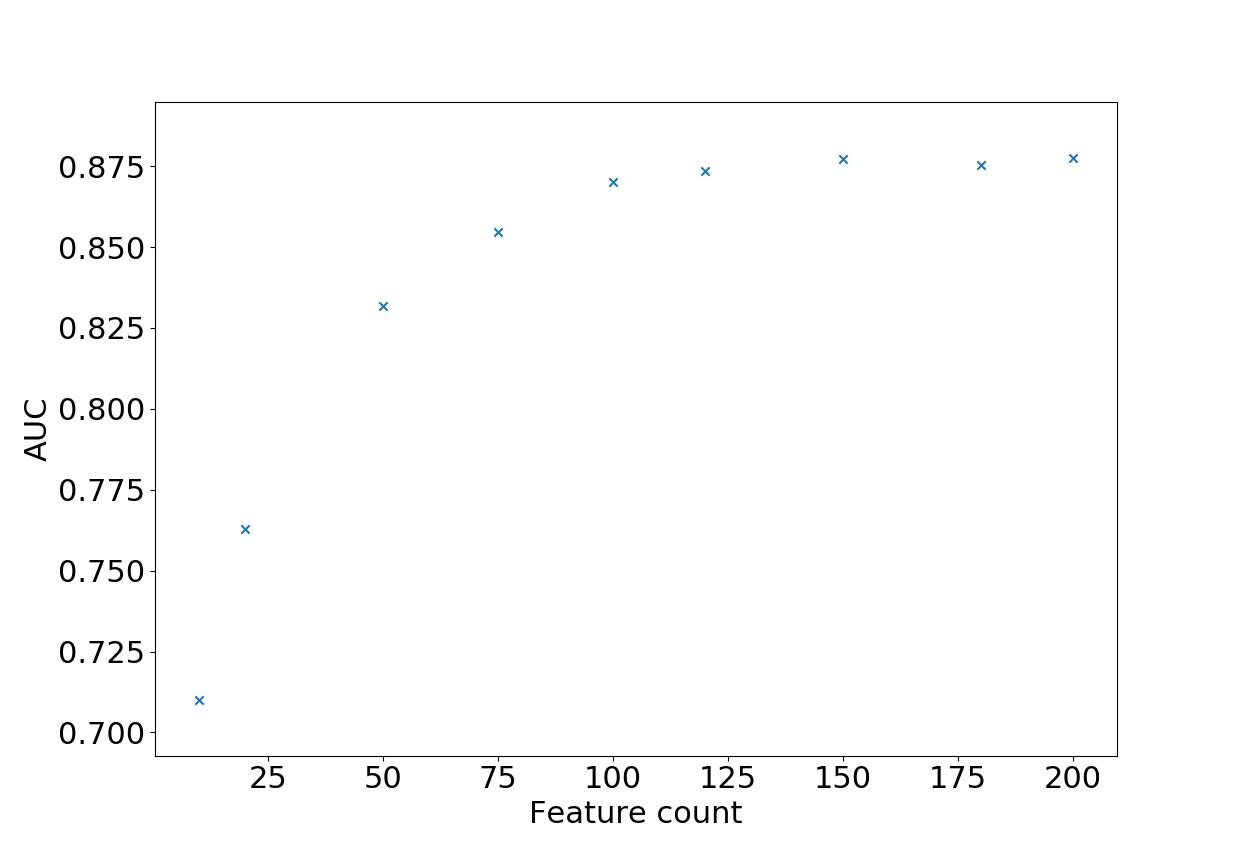
\includegraphics[width=0.95\textwidth]{xgboost/feature_count.png}
    \caption{Wartość miary AUC w zależności od liczby wybranych cech}
    \label{fig:xgboost_feature_count}
\end{figure}

\begin{table}[h]
    \centering
    \begin{tabular}{|l|c|c|c|c|c|c|c|c|c|}
        \hline
        Liczba cech & 10 & 20 & 50 & 75 & 100 & 120 & 150 & 180 & \textbf{200} \\ \hline
        AUC & 0.7101 & 0.7628 & 0.8319 & 0.8548 & 0.8670 & 0.8734 & 0.8772 & 0.8755 & \textbf{0.8776} \\ \hline
    \end{tabular}
    \caption{Wartość miary AUC w zależności od liczby wybranych cech}
    \label{tab:xgboost_feature_count}
\end{table}

Przeprowadzone testy potwierdzają tezę zespołu od wstępnego przetwarzania danych, cechy są od siebie niezależne, wybranie wszystkich zatem nie pogarsza wyniku. Wręcz przeciwne, daje to w tym przypadku najlepszy wynik, chociaż wszystkie wyniki dla liczby cech większej równej 120 są raczej porównywalnie dobre. Do dalszych analiz będą więc używane wszystkie cechy, żadnej nie trzeba pomijać.

Patrząc na to jak się model uczył (rysunek \ref{fig:xgboost_training_overfitting}) widać niestety, że model jest przetrenowany, dla zestawu treningowego AUC osiąga prawie 1.0, podczas gdy dla walidacyjnego nie potrafi osiągnąć 0.88. Podobnie jest z funkcją straty, model znacznie lepiej uczy się zbioru treningowego. Najwyraźniej domyślna maksymalna wysokość drzew jest zbyt duża, dlatego ten parametr był następnie badany.

\begin{figure}[h]
    \centering
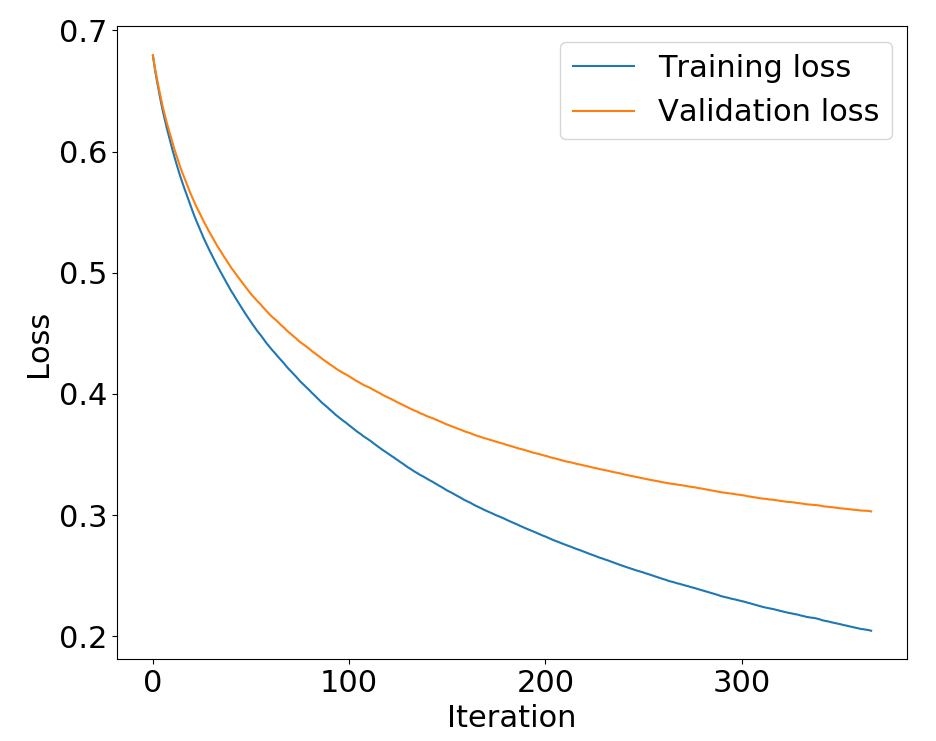
\includegraphics[width=0.45\textwidth]{xgboost/overfitting_loss.png}
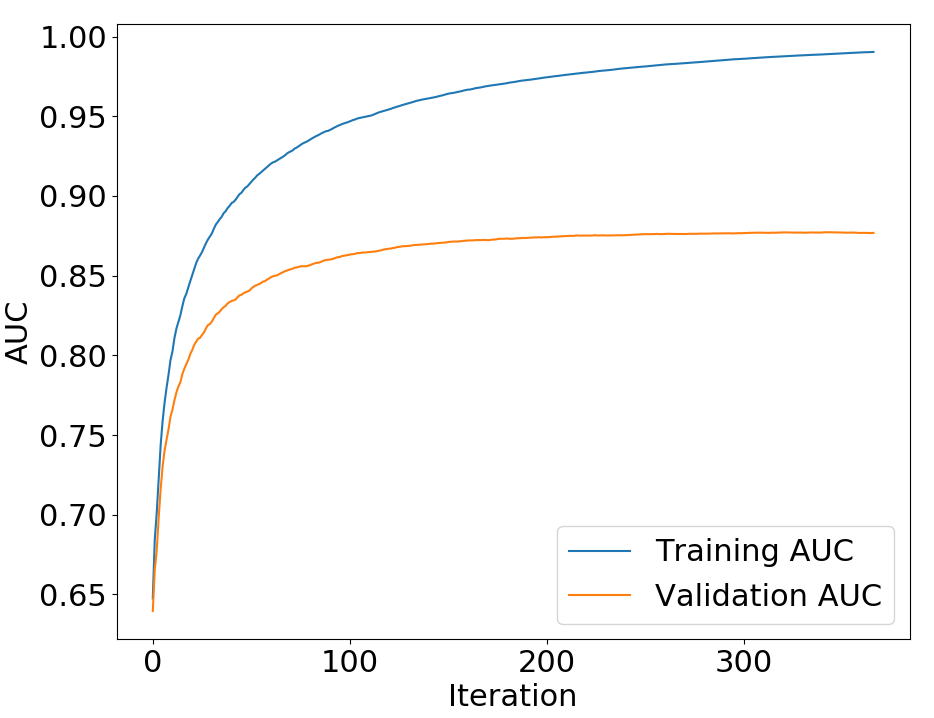
\includegraphics[width=0.45\textwidth]{xgboost/overfitting_auc.png}
    \caption{Wartości funkcji straty i miary AUC w zależności od iteracji dla domyślnych parametrów}
    \label{fig:xgboost_training_overfitting}
\end{figure}

\subsubsection{Wysokość drzew i min\_child\_weight}

Faktycznie analizując wyniki z tabeli \ref{tab:xgboost_depth} możemy zauważyć, że mniejsze wysokości znacznie lepiej się sprawują niż domyślna wartość. Widać, że dobrany model był zbytnio złożony, po trenowaniu nie był wystarczająco ogólny. Tą samą tendencję widać dla parametru min\_child\_weight, tu dla większych wartości wyniki są trochę lepsze. Większe wartości tego parametru oznaczają, ze drzewa będą miały mniej liści, czyli model będzie mniej skomplikowany.

\begin{table}[h]
    \centering
    \begin{tabular}{|l|c|c|c|c|c|c|c|c|c|}
        \hline
         & &  \multicolumn{8}{c|}{min\_child\_weight}  \\ \hline
        \multirow{6}{*}{Wysokość} & & 0.5  & 1 & 2 & 4 & 6 & 8 & 10 & 12 \\ \cline{2 - 10}
        & 1 & 0.8965 & 0.8965 & 0.8965 & 0.8965 & 0.8965 & \textbf{0.8970} & 0.8964 & \textbf{0.8970} \\ \cline{2-10}
        & 2 & 0.8931 & 0.8931 & 0.8929 & 0.8934 & 0.8926 & 0.8925 & 0.8930 & 0.8931 \\ \cline{2 - 10} 
        & 3 & 0.8897 & 0.8894 & 0.8890 & 0.8890 & 0.8884 & 0.8883 & 0.8885 & 0.8879 \\ \cline{2 - 10} 
        & 4 & 0.8837 & 0.8835 & 0.8831 & 0.8841 & 0.8839 & 0.8835 & 0.8832 & 0.8837 \\ \cline{2 - 10} 
        & 5 & 0.8778 & 0.8776 & 0.8783 & 0.8771 & 0.8779 & 0.8759 & 0.8799 & 0.8778 \\ \cline{2 - 10} 
        & 6 & 0.8698 & 0.8697 & 0.8693 & 0.8716 & 0.8708 & 0.8705 & 0.8794 & 0.8717 \\ \hline

    \end{tabular}
    \caption{Wartości miary AUC dla różnych maksymalnych wysokości drzew i wartości parametru min\_child\_weight}
    \label{tab:xgboost_depth}
\end{table}

Do dalszych analiz została wybrana maksymalna wysokość drzew równa jeden, a wartość parametru min\_child\_weight równa osiem. Patrząc na proces uczenia dla drzew o wysokości jeden (rysunek \ref{fig:xgboost_training_depth1}, widać że zjawisko przetrenowania zostało znacznie zmniejszone, miara AUC dla zbioru treningowego nie osiąga już 1.0, jest bliższa miary dla zbioru walidacyjnego. Co więcej, im niższe drzewa, tym mniej trwa jedna iteracja algorytmu, za to liczba iteracji znacznie rośnie (prawie 1200 zamiast około 350). 

\begin{figure}[h]
    \centering
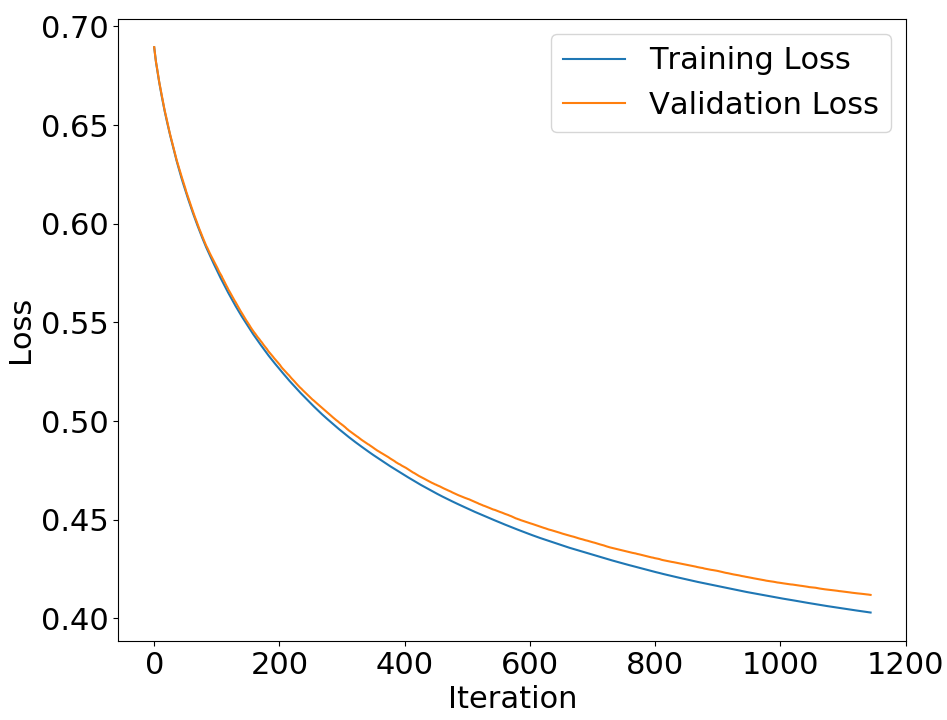
\includegraphics[width=0.48\textwidth]{xgboost/depth1_loss.png}
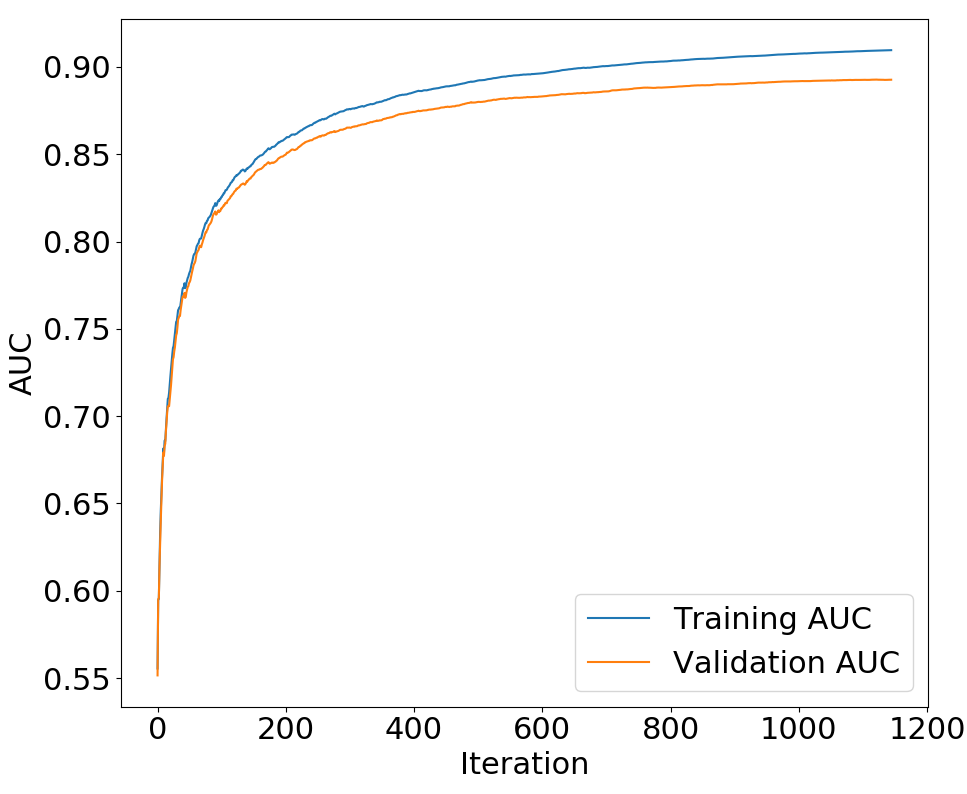
\includegraphics[width=0.45\textwidth]{xgboost/depth1_auc.png}
    \caption{Wartości funkcji straty i miary AUC w zależności od iteracji dla drzew o maksymalnej wysokości 1}
    \label{fig:xgboost_training_depth1}
\end{figure}

\subsubsection{Colsample\_by\_tree i subsample}

Kolejne parametry, które sterują stopniem skomplikowania modelu są colsample\_by\_tree i subsample. W tablicy \ref{tab:xgboost_sample} są przedstawione dokładne wartości miary AUC dla różnych kombinacji tych parametrów.

\begin{table}[h]
    \centering
    \begin{tabular}{|l|c|c|c|c|c|}
        \hline
         & &  \multicolumn{4}{c|}{colsample\_by\_tree}  \\ \hline
        \multirow{6}{*}{subsample} & & 0.4 & 0.6 & 0.8 & 1.0 \\ \cline{2 - 6}
& 0.4 & 0.8964 & 0.8975 & 0.8967 & 0.8950 \\ \cline{2 - 6} 
& 0.6 & 0.8964 & 0.8950 & 0.8962 & 0.8966 \\ \cline{2 - 6} 
& 0.8 & 0.8973 & 0.8976 & 0.8965 & \textbf{0.8977} \\ \cline{2 - 6} 
& 1 & 0.8970 & 0.8963 & 0.8970 & 0.8970 \\ \hline

    \end{tabular}
    \caption{Wartości miary AUC dla różnych wartości colsample\_by\_tree i subsample}
    \label{tab:xgboost_sample}
\end{table}

Widać wyraźnie, że mniejsze wartości parametrów nie poprawiają jakości modelu, to oznacza że poprzez zastosowanie wielu niskich drzew, model jest już wystarczająco ogólny, nie trzeba przy trenowaniu losowo pomijać kolumn lub wierszy. Najlepszy wynik został uzyskany dla subsample równego 0.8 i colsample\_by\_tree równego 1.0. Oznacza to że przy tworzeniu kolejnego drzewa brane są pod uwagę wszystkie kolumny i losuje się 80\% z wierszy. Dla tych wartości parametrów zostały też przeprowadzone kolejne analizy.

\subsubsection{Współczynnik uczenia eta}

Ostatnim optymalizowanym parametrem był współczynnik uczenia. Szczególnie mniejsze wartości mogą być tutaj ciekawe, mogę spowodować, że algorytm przy schodzeniu po gradiencie znajdzie jakieś minimum, które wcześniej pomijał przez wykonywanie zbyt dużych kroków. Wyniki można zobaczyć w tablicy \ref{tab:xgboost_eta}.

\begin{table}[h]
    \centering
    \begin{tabular}{|c|c|}
    \hline
        eta & AUC \\ \hline
        0.5 & 0.8940 \\ \hline 
        0.2 & 0.8977 \\ \hline 
        0.15 & \textbf{0.8978} \\ \hline 
        0.1 & 0.8971 \\ \hline 
        0.05 & 0.8976 \\ \hline 
        0.02 & 0.8967 \\ \hline 
        0.01 & 0.8969 \\ \hline 
        0.005 & 0.8949 \\ \hline 
        0.001 & 0.5554 \\ \hline
    \end{tabular}
    \caption{AUC dla różnych wartości współczynnika uczenia eta}
    \label{tab:xgboost_eta}
\end{table}

Zgodnie z oczekiwaniami, zwiększenie współczynnika uczenia nie poprawiło jakości modelu. Tak samo zbyt małe wartości, jak na przykład 0.001 powodowały za wolne uczenie i przez to zwracały niedouczony model. Dla pośrednich wartości (0.2, 0.15, 0.1, 0.05, 0.02, 0.01) został przeprowadzony kolejny eksperyment, mianowicie liczba iteracji, po której uczenie jest przerywane, jeżeli nie nastąpiła poprawa miary AUC, została zwiększona z 25 do 1000. To ma dać szansę mniejszym współczynnikom uczenia, które po prostu czasami potrzebują więcej niż 25 iteracji, aby znaleźć odpowiedni kierunek w gradiencie, wzdłuż którego nastąpi poprawa modelu. Wyniki tego eksperymentu są przedstawione w tabeli \ref{tab:xgboost_eta_longer}.

\begin{table}[h]
    \centering
    \begin{tabular}{|c|c|}
    \hline
        eta & AUC \\ \hline
        0.2 & 0.8977 \\ \hline 
        0.15 & 0.8978 \\ \hline 
        0.1 & \textbf{0.8980} \\ \hline 
        0.05 & \textbf{0.8980} \\ \hline 
        0.02 & 0.8979 \\ \hline 
        0.01 & \textbf{0.8980} \\ \hline 
    \end{tabular}
    \caption{AUC dla różnych wartości współczynnika uczenia eta i dłuższym okresie uczenia}
    \label{tab:xgboost_eta_longer}
\end{table}

Widać, że w tym przypadku niskie współczynniki uczenia lepiej wypadają, niż wtedy gdy miały mniejszą liczbę iteracji, aby poprawić model, niemniej jednak wzięcie niższego eta niż 0.1 nie ma sensu, wydłuża to znacznie uczenie bez znaczącej poprawy.

\subsubsection{Podsumowanie boostingu}

W tabeli \ref{tab:xgboost_best_params} zostały przedstawione ostatecznie wybrane parametry modelu. Z procesu wyznaczania tych parametrów, można wywnioskować, że najważniejsze było odpowiednie dobranie maksymalnej wysokości drzew, to pozwoliło na tyle uprościć model, żeby podczas treningu nadal pozostał ogólny i tym samym zredukować zjawisko przetrenowania. Drugim wnioskiem jest to, że im więcej parametrów już zostało ustalonych, tym mniejsze poprawy wnosiły kolejne zmiany innych parametrów. 

\begin{table}[h]
    \centering
    \begin{tabular}{l | c }
        Parametr & Wartość \\ \hline
        scale\_pos\_weight & 9 \\
        liczba cech & 200 \\
        maks. wysokość & 1 \\
        min\_child\_weight & 8 \\
        subsample & 0.8 \\
        colsample\_by\_tree & 1 \\
        eta & 0.1 \\
        % alfa & 0 \\
        % lambda & 1 \\
    \end{tabular}
    \caption{Najlepsze wartości hiperparametrów użytych w boostingu drzew}
    \label{tab:xgboost_best_params}
\end{table}

Na zestawie testowym udostępnionym przez platformę kaggle (bez etykiet, jakość rozwiązania jest oceniana przez załadowanie pliku csv z wyjściem modelu na stronie internetowej), model korzystający z wyżej wymienionych parametrów uzyskał miarę AUC równą 0.8978, czyli bardzo zbliżoną do tego, co udało się uzyskać na zbiorze walidacyjnym. Niestety model był gotowy dopiero po zakończeniu konkursu, w chwili zakończenia konkursu najlepszy nasz model korzystający z boostingu drzew uzyskał wynik 0.8958, co dało 5244 pozycję z 8802 uczestników konkursu.

\subsubsection{Instrukcja uruchomienia boostingu}

Boosting został zaimplementowany w Pythonie i można go uruchomić jako aplikację konsolową:

\begin{lstlisting}
boost.py [-h] [--seed=SEED] [--infer=INFER] [--ratio=RATIO]
[--results=RESULTS] [-c CONFIG] [-m MODEL] input_data
\end{lstlisting}

Znaczenie parametrów:

\begin{itemize}
    \item -h: wyświetlenie pomocy
    \item --seed: seed dla generatora liczb losowych, używany aby mieć powtarzalne wyniki (domyślnie None, wtedy seed nie będzie uzywany, dla każdego uruchomienia będa inne wyniki)
    \item --infer: ścieżka do zbioru testowego, jeśli zostanie podana ta opcja, to zamiast uczyć model, uruchamiany jest tryb predykcji i tworzony plik submission.csv z wynikami dla podanego zbioru danych. Ten plik potem można przesłać do serwerów kaggle w ramach sprawdzenia jakości klasyfikatora.
    \item --ratio: liczba rzeczywista, stosunek wierszy używanych do treningu do wszystkich wierszy. Domyślnie 0.8, czyli 80\% wierszy tworzy zbiór uczący, reszta (20 \%) zbiór walidacyjny.
    \item --results: ścieżka do pliku csv gdzie zostaną dopisane wyniki modelu (jego parametry oraz wartości miar takich jak AUC). Jeśli plik nie istnieje to zostanie stworzony. Domyślnie \verb"results.csv".
    \item -c: ścieżka do pliku json z konfiguracją modelu. Przykładowe pliki konfiguracyjne są dostępne w folderze boost-configs. Domyślnie \verb"boost-configs/default.json".
    \item -m: ścieżka do modelu, w trybie treningu jest to ścieżka pod którą zostanie zapisany wytrenowany model, w trybie predykcji ścieżka do modelu wykorzystanego do predykcji.
    \item input{\_}data: ścieżka do pliku csv w którym znajdują się dane treningowe. Jedyny tak naprawdę wymagany parametr, nie posiada domyślnej wartości, może być podany w dowolnym miejscu. Trzeba również podać w trybie predykcji, żeby skrypt dobrze przeskalował dane wejściowe.
\end{itemize}

\noindent Przykładowe wywołania:

\noindent Trening:
\begin{lstlisting}
./boost.py ../data/train.csv --seed=42 -m new.model 
-c boost-configs/best.json --results=results.csv
\end{lstlisting}

\noindent Predykcja:
\begin{lstlisting}
./boost.py ../data/train.csv --seed=42 -m best.model
--infer=../data/test.csv
\end{lstlisting}


\subsection{Bayesian Gaussian mixture model}
\subsubsection{Opis metody}

Bayesian model polega na wykorzystaniu twierdzenia Bayesa do stworzenia klasyfikatora, którego model został wyprowadzony przy użyciu tego twierdzenia. Gaussian mixture model zakłada, że w zbiorze danych istnieje skończona liczba podzbiorów, które mogą zostać przybliżone rozkładem Gaussa. Do obliczeń została wykorzystana implementacja z pakietu sklearn.mixture.GaussianMixture. \\
Problem, który rozwiązujemy ma 2 niezbalansowane klasy i 200 cech, które zakładamy, że są niezależne względem siebie. Modelujemy $Y$ jako Bernoulli, gdzie 0 - fałsz, 1 - prawda, podczas gdy cechy $X_{0}, X_{1}, ... , X_{199}$ są ciągłymi zmiennymi losowymi. Teraz trzeba przypomnieć twierdzenia Bayesa:
\begin{equation}
    p_{Y|X_0,X_1,\ldots,X_{199}}(y|x_0,x_1,\ldots,x_{199})=\frac{p_Y(y)\prod_{i=0}^{199}f_{X_i|Y}(x_i|y)}{\sum_{y'=0}^1p_Y(y')\prod_{i=0}^{199}f_{X_i|Y}(x_i|y')}
\end{equation}
gdzie $p_Y(y)$ będzie proporcją między 2 klasami, a prawdopodobieństwo $f_{X_i|Y}(x_i|y)$ będzie uzyskane przy pomocy Gaussian mixture model.

\subsubsection{Trenowanie modelu}
Użycie sklearn.mixture.GaussianMixture pozostawia nam dopasowanie 2 hiperparametrów:
\begin{itemize}
    \item \textbf{n\_components} - liczba składowych rozkładów normalnych
    \item \textbf{reg\_covar} - parametr regulujący dodawany do diagonali macierzy kowariancji.
\end{itemize}

Były sprawdzane różne wartości parametrów metodą hyperparameter grid search. Do porównywania wyników dla poszczególnych parametrów została użyta miara AUC-ROC dla zbioru walidacyjnego i treningowego. Poniżej przedstawione są najlepsze wyniki przeszukiwania parametrów (pod względem wyniku dla zbioru walidacyjnego):

\begin{table}[h]
    \centering
    \begin{tabular}{|c|c|c|c|}
    \hline
        component\_number & reg\_covar & AUC\_train & AUC\_val \\ \hline
        15 & 0.01 & 0.9105 & 0.9006 \\ \hline 
        10 & 0.01 & 0.9091 & 0.8997 \\ \hline 
        20 & 0.01 & 0.9112 & 0.8994 \\ \hline 
        5 & 0.01 & 0.9052 & 0.8990 \\ \hline 
        5 & 0.0001 & 0.8971 & 0.8889 \\ \hline 
    \end{tabular}
    \caption{AUC treningowe i walidacyjne dla różnych wartości współczynników component\_number i reg\_covar}
    \label{tab:gaussian_mix_gridsearch}
\end{table}

Najlepiej sprawdza się tutaj reg\_covar o wartości około 0.01 i component\_number o wartości 15, co daje wynik 0.9006 dla zbioru walidacyjnego. 

Ze względu na duże niezbalansowanie klas, zostały także przeprowadzone eksperymenty po przeprowadzeniu oversamplingu, a także dla danych po użyciu undersamplingu. Do obydwu technik został zastosowany pakiet \textit{imblearn}.

\begin{table}[h]
    \centering
    \begin{tabular}{|c|c|c|c|}
    \hline
        component\_number & reg\_covar & AUC\_train & AUC\_val \\ \hline
        15 & 0.01 & 0.9137 & 0.9053 \\ \hline 
        20 & 0.01 & 0.9148 & 0.9053 \\ \hline 
        10 & 0.01 & 0.9118 & 0.9048 \\ \hline 
        5 & 0.01 & 0.9063 & 0.9023 \\ \hline 
        5 & 0.001 & 0.9021 & 0.8989 \\ \hline 
    \end{tabular}
    \caption{AUC treningowe i walidacyjne dla różnych wartości współczynników component\_number i reg\_covar po undersamplingu}
    \label{tab:gaussian_mix_gridsearch_undersampling}
\end{table}

\begin{table}[h]
    \centering
    \begin{tabular}{|c|c|c|c|}
    \hline
        component\_number & reg\_covar & AUC\_train & AUC\_val \\ \hline
        20 & 0.01 & 0.9137 & 0.9104 \\ \hline 
        15 & 0.01 & 0.9137 & 0.9101 \\ \hline 
        10 & 0.01 & 0.9137 & 0.9087 \\ \hline 
        5 & 0.01 & 0.9137 & 0.9054 \\ \hline 
        5 & 0.0001 & 0.9137 & 0.8959 \\ \hline 
    \end{tabular}
    \caption{AUC treningowe i walidacyjne dla różnych wartości współczynników component\_number i reg\_covar po oversamplingu}
    \label{tab:gaussian_mix_gridsearch_oversampling}
\end{table}

Na podstawie powyższych tabel możemy stwierdzić, że najlepiej ustawić reg\_covar na wartość około 0.01 we wszystkich przypadkach. Component\_number zaś wacha się pomiędzy 15 a 20, możliwe że najlepsza byłaby jakaś wartość pomiędzy. Zarówno po oversamplingu jak i po undersamplingu, wyniki metody są lepsze w przypadku zbioru walidacyjnego. Najlepsze wyniki osiągane są po oversamplingu, jednak nie są dużo lepsze niż po undersamplingu, więc nie jest pewne, że modele wytrenowane na zbiorze po oversamplingu osiągną lepsze rezultaty także w przypadku konkursowego zbioru danych. 

\subsubsection{Wyniki}

Po zamieszczeniu wyników z najlepiej radzących sobie zestawów parametrów zarówno dla modeli wytrenowanych po oversamplingu jak i undersamplingu danych, oraz bez korzystania z żadnego z nich, najlepsze wyniki w konkursie osiągnęte zostały po użyciu oversamplingu osiągając wynik 0.89251, trochę gorszy niż wynik, który został osiągnięty dla zbioru walidacyjnego. Dało to pozycję 5656 z 8802 uczestników konkursu.

\subsubsection{Instrukcja uruchomienia}

Bayesian Gaussian mixture model został zaimplementowany w Pythonie i można go uruchomić jako aplikację konsolową:

\begin{lstlisting}
gaussian_mixture.py [-h] [--train_data=PATH] [--data=PATH] [--seed=SEED]
[--data_balancing=O/U] [--is_only_training=true/false] [--reg_covar=FLOAT] [--is_grid_search=true/false] [--output=PATH]
\end{lstlisting}

Znaczenie parametrów:

\begin{itemize}
    \item -h: wyświetlenie pomocy
    \item train{\_}data: ścieżka do pliku csv w którym znajdują się dane treningowe. Domyślnie: ../data/train.csv
    \item data: ścieżka do pliku csv w którym znajdują się dane. Domyślnie: ../data/test.csv
    \item --seed: seed dla generatora liczb losowych, używany aby mieć powtarzalne wyniki. Domyślnie: 12415.
    \item data{\_}balancing: czy używany będzie oversampling (O) lub undersampling (U). Domyślnie: O
    \item is{\_}only{\_}training: ustawiony na true, jeśli ma zostać wykonany tylko trening modelu. Domyślnie: false
    \item component{\_}number: liczba komponentów gaussian mixture. Domyślnie: 5
    \item reg{\_}covar: nieujemny parametr regulujący dodawany do diagonali macierzy kowariancji. Domyślnie: 1e-2
    \item is{\_}grid{\_}search: jeśli jest ustawiony na true, wykonuje grid search dla stałych parametrów component{\_}number i reg{\_}covar. Domyślnie: false
    \item output: ścieżka do pliku wyjściowego. Domyślnie: gauss{\_}mix{\_}output.csv
\end{itemize}

\noindent \textbf{Przykładowe wywołania:}\\

\noindent Trening wraz z predykcją:
\begin{lstlisting}
./gaussian_mixture.py --seed=125152 --train_data=../data/train.csv --data=../data/test.csv --data_balancing=o --component_number=3 --reg_covar=1e-3 --output=output.csv
\end{lstlisting}

\noindent Grid search:
\begin{lstlisting}
./gaussian_mixture.py--train_data=../data/train.csv --data=../data/test.csv --data_balancing=o --component_number=7 --reg_covar=1e-2 --is_grid_search True --output=output.csv
\end{lstlisting}


\section{Wyniki i podsumowanie}

\newpage

\section{Bibliografia}
\begin{thebibliography}{9}

\bibitem{santanderkaggle}
\url{https://www.kaggle.com/c/santander-customer-transaction-prediction}
\bibitem{xgboost}
\url{https://github.com/dmlc/xgboost}
\bibitem{gradboosting}
\url{https://medium.com/mlreview/gradient-boosting-from-scratch-1e317ae4587d}
\bibitem{sklearn}
\url{https://scikit-learn.org}

\bibitem{exampple}
  John Example,
  \textit{Example title}.
  Exampler,
  1996.

\end{thebibliography}

\end{document} 